\documentclass[11pt,a4paper]{article}

\usepackage{fontspec}
\usepackage{xunicode}
\usepackage{xltxtra}
\usepackage{polyglossia}
\usepackage{amsmath}
\usepackage{amsfonts}
\usepackage{amssymb}
\usepackage{graphicx}
\usepackage[left=2cm,right=2cm,top=2cm,bottom=2cm]{geometry}
\usepackage{afterpage}
\usepackage{xcolor}
\usepackage{pagecolor}
\usepackage{mathtools}
%\usepackage{fancyhdr}
\usepackage{hyperref}
\usepackage{blindtext}
\usepackage{mahjong}
\usepackage{amsthm}
\usepackage{chngcntr}
\usepackage{tikz}

\usepackage{stmaryrd}
\let\stmaryrdLightning\lightning


\defaultfontfeatures{Mapping=tex-text}
%\setmainfont{???}
\setdefaultlanguage{german}
\definecolor{114F9D}{HTML}{114F9D}
\author{Zehao Gao}

\newtheorem{theorem}{Satz}[section]

\newtheorem{corollary}{Korollar}[theorem]

\newtheorem{lemma}[theorem]{Lemma}

\newtheorem{conclusion}[theorem]{Folgerung}

\theoremstyle{definition}
\newtheorem{definition}{Definition}[section]

\theoremstyle{remark}
\newtheorem*{remark}{Bemerkung}

\theoremstyle{remark}
\newtheorem{exmp}{Beispiel}[section]

\theoremstyle{remark}
\newtheorem*{solution}{Lösung}

\renewcommand{\frac}{\dfrac}

\counterwithin*{equation}{section}
\counterwithin*{equation}{subsection}
%\counterwithin*{equation}{paragraph}

\begin{document}

\begin{titlepage}

\pagecolor{114F9D}\afterpage{\nopagecolor}

\begin{center}

\null

\vspace{50pt}

\textcolor{white}%LARGE TITLE
{
\Huge Übungen \& Hausaufgaben\\
\Huge \textbf{Analysis}\\
\vspace{8pt}
\Large WS2022/23-SS2023\\
}

\vspace{8pt}

\begin{figure}[h]%Cauchy portrait
\centering
{
\fboxsep=0pt
\fboxrule=3pt
\fcolorbox{white}{white}{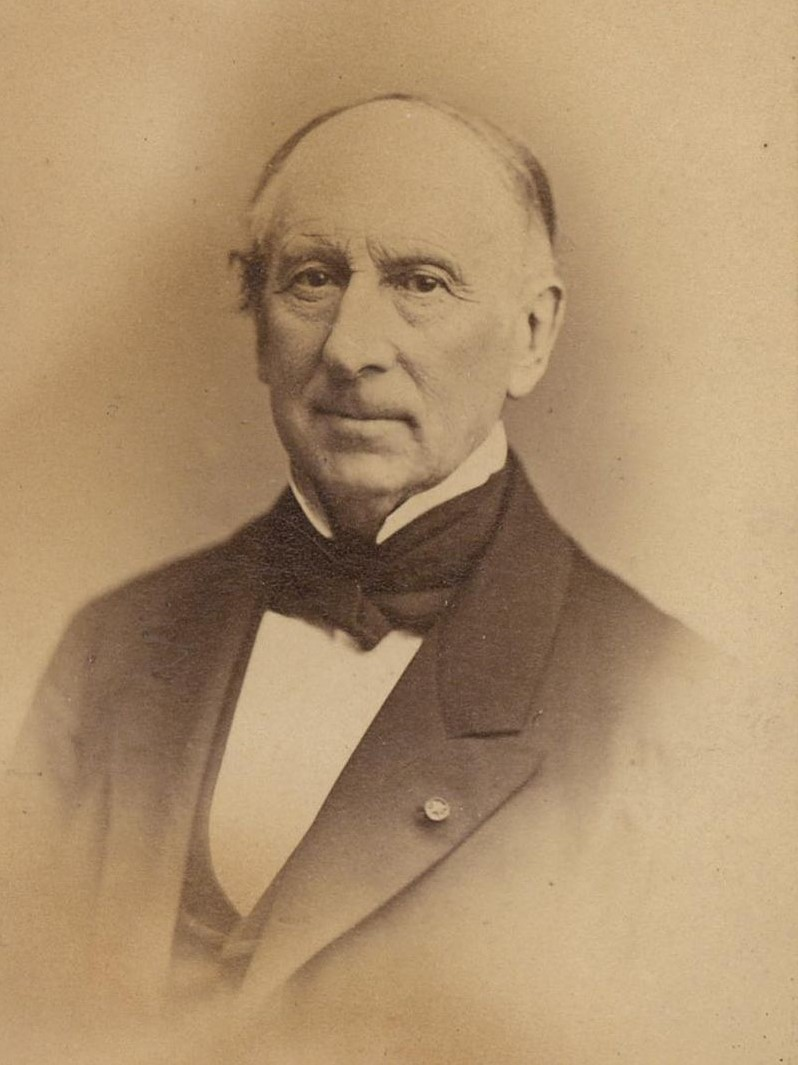
\includegraphics[width=10cm]{./pics/Cauchy.jpg}}
}
\end{figure}

\vspace{4pt}

\textcolor{white}
{
\Huge Zehao Gao\\
\large M.Nummer 5052835\\
%\large Übungsgruppe Mi 5Ds Wang
}

\begin{figure}[b]
\centering
\textcolor{white}
{
\Large \LaTeX
}
\end{figure}

\end{center}

\end{titlepage}


\newpage

\tableofcontents

\newpage

\section{1. Übungsblatt: $Aussagen\ und\ Quantoren$}

\subsection{Aufgabe 1.1}

\paragraph{(a)}
\begin{proof}
$ $\newline
Sei $p$ $wahr$:
\begin{equation}
p\ wahr\Rightarrow\neg p\ falsch
\end{equation}
\begin{equation}
\Rightarrow (p\wedge\neg p)\ falsch
\end{equation}
\begin{equation}
\Rightarrow \neg(p\wedge\neg p)\ wahr
\end{equation}\\
Sei $p$ $falsch$:
\begin{equation}
p\ falsch\Rightarrow\neg p\ wahr
\end{equation}
\begin{equation}
\Rightarrow (p\wedge\neg p)\ falsch
\end{equation}
\begin{equation}
\Rightarrow \neg(p\wedge\neg p)\ wahr
\end{equation}\\
$Folgerung:$ Diese Formel ist Tautologie.
\end{proof}

\paragraph{(b)}
\begin{proof}
$ $\newline
\begin{center}
\begin{tabular}{||c|c||c|c|c|c|c|c||}
\hline
$p$ & $q$ & $\neg p$ & $\neg q$ & $p\wedge q$ & $\neg(p\wedge q)$ & $(\neg p)\vee (\neg q)$ & $\neg(p\wedge q)\Leftrightarrow((\neg p)\vee (\neg q))$ \\
\hline
\hline
$w$ & $w$ & $f$ & $f$ & $w$ & $f$ & $f$ & $w$ \\
%\hline
$w$ & $f$ & $f$ & $w$ & $f$ & $w$ & $w$ & $w$ \\
%\hline
$f$ & $w$ & $w$ & $f$ & $f$ & $w$ & $w$ & $w$ \\
%\hline
$f$ & $f$ & $w$ & $w$ & $f$ & $w$ & $w$ & $w$ \\
\hline
\end{tabular}
\end{center}
$Folgerung:$ Diese Formel ist Tautologie.
\end{proof}

\paragraph{(c)}
\begin{proof}
$ $\newline
\begin{center}
\begin{tabular}{||c|c||c|c|c|c|c||}
\hline
$p$ & $q$ & $\neg p$ & $\neg q$ & $p\Rightarrow q$ & $(p\Rightarrow q)\wedge (\neg q)$ & $((p\Rightarrow q)\wedge (\neg q))\Rightarrow (\neg p)$ \\
\hline
\hline
$w$ & $w$ & $f$ & $f$ & $w$ & $f$ & $w$ \\
%\hline
$w$ & $f$ & $f$ & $w$ & $f$ & $f$ & $w$ \\
%\hline
$f$ & $w$ & $w$ & $f$ & $w$ & $f$ & $w$ \\
%\hline
$f$ & $f$ & $w$ & $w$ & $w$ & $w$ & $w$ \\
\hline
\end{tabular}
\end{center}
$Folgerung:$ Diese Formel ist Tautologie.
\end{proof}

\newpage

\paragraph{(d)}
\begin{proof}
$ $\newline
\begin{center}
\begin{tabular}{||c|c|c||c|c|c|c|c|c||}
\hline
$p$ & $q$ & $r$ & $q\wedge r$ & $p\vee q$ & $p\vee r$ & $p\vee (q\wedge r)$ & $(p\vee q)\wedge (p\vee r)$ & $(p\vee (q\wedge r))\Leftrightarrow ((p\vee q)\wedge (p\vee r))$ \\
\hline
\hline
$w$ & $w$ & $w$ & $w$ & $w$ & $w$ & $w$ & $w$ & $w$ \\

$w$ & $w$ & $f$ & $f$ & $w$ & $w$ & $w$ & $w$ & $w$ \\

$w$ & $f$ & $w$ & $f$ & $w$ & $w$ & $w$ & $w$ & $w$ \\

$w$ & $f$ & $f$ & $f$ & $w$ & $w$ & $w$ & $w$ & $w$ \\

$f$ & $w$ & $w$ & $w$ & $w$ & $w$ & $w$ & $w$ & $w$ \\

$f$ & $w$ & $f$ & $f$ & $w$ & $f$ & $f$ & $f$ & $w$ \\

$f$ & $f$ & $w$ & $f$ & $f$ & $w$ & $f$ & $f$ & $w$ \\

$f$ & $f$ & $f$ & $f$ & $f$ & $f$ & $f$ & $f$ & $w$ \\
\hline
\end{tabular}
\end{center}
$Folgerung:$ Diese Formel ist Tautologie.
\end{proof}

\paragraph{(e)}
$ $\newline
Die Negation von Satz "Satz vom Widerspruch" ist einfach eine Kontradiktion:
\begin{equation*}
\neg (\neg (p\wedge \neg p))\Leftrightarrow p\wedge \neg p\ \ (stets\ falsch)
\end{equation*}

\newpage

\subsection{Aufgabe 1.2}

\paragraph{}
\begin{solution}
$ $\newline
Wir vereinfachen nun die Formel $(\neg ((p\Rightarrow (q\Rightarrow p))\wedge p)\vee (q\Rightarrow q))\Rightarrow p$ \\
Nach Wahrheitstabelle gilt es:
\begin{equation*}
(p\Rightarrow (q\Rightarrow p))\Leftrightarrow p,\ (q\Rightarrow q)\Leftrightarrow q
\end{equation*}
Damit vereinfachen wir die Formel zu:
\begin{equation}
(\neg (p\wedge p)\vee q)\Rightarrow p
\end{equation}
Nach Wahrheitstabelle gilt es:
\begin{equation*}
(p\vee p)\Leftrightarrow p
\end{equation*}
Damit vereinfachen wir die Formel zu:
\begin{equation}
(\neg p\vee q)\Rightarrow p
\end{equation}
Nach Priorität von Verknüpfungen können wir noch vereinfachen:
\begin{equation}
\neg p\vee q\Rightarrow p
\end{equation}
\end{solution}
\begin{remark}
$(a\Rightarrow b)\Leftrightarrow(\neg a\wedge b)$
\end{remark}

\newpage

\subsection{Aufgabe 1.3}

\paragraph{(a)}
\begin{solution}
$ $\newline
$(x\in\mathbb{R})\wedge(x^2=1)\Leftrightarrow (x=1)\wedge(x=-1)$
\end{solution}
\textbf{Negation}\\
$\forall x\in\mathbb{R}$ und $x^2=1$ $\Rightarrow(x=1)\vee(x=-1)$

\paragraph{(b)}
\begin{solution}
$ $\newline
$\neg(\exists x\in\mathbb{R})\Rightarrow(x^2=-1)$
\end{solution}
\textbf{Negation}\\
$(\exists x\in\mathbb{R})\Rightarrow(x^2=-1)$
\begin{remark}
Es gilt auch $\nexists x\in\mathbb{R}$
\end{remark}

\paragraph{(c)}
\begin{solution}
$ $\newline
$(x\in\mathbb{N})\wedge((\frac{x}{6}\in\mathbb{Z})\vee((\frac{x}{4}\in\mathbb{Z})\wedge(\frac{x}{9}\in\mathbb{Z})))\Rightarrow(\frac{x}{2}\in\mathbb{Z})\wedge(\frac{x}{3}\in\mathbb{Z})$
\end{solution}
\textbf{Negation}\\
$\exists n\in\mathbb{N}:\ (6|n)\vee((4|n)\wedge(9|n))\Rightarrow(2\nmid n)\vee(3\nmid n)$
\begin{remark}
$(a|b)$ bedeutet: $b$ durch $a$ teilbar
\end{remark}

\paragraph{(d)}
\begin{solution}
$ $\newline
$(\forall x\in\mathbb{N})\Rightarrow(\exists y\in\mathbb{P})\wedge(y>x)$
\end{solution}
\textbf{Negation}\\
$\exists n\in\mathbb{N}\ \forall p\in\mathbb{P}:\ p\leq n$

\paragraph{(e)}
\begin{solution}
$ $\newline
$(M\subset\mathbb{Z})\Rightarrow(\exists!k\in M)\wedge(\forall g\in M\setminus k)\wedge(g>k)$
\end{solution}
\textbf{Negation}\\
$\exists M\subset\mathbb{N}:\ \forall m\in\ M\ \exists n\in\ M\setminus\{m\}:\ m\geq n$\\
oder\\
$\exists m_1,\ m_2\in\ M,\ m_1\neq m_2:\ m_1<n,\ m_2<n$

\newpage

\subsection{Aufgabe 1.4}
Wir nennen: $G,\ H,\ N,\ D,\ R,\ Z,\ S$\\
\begin{align}
H\Rightarrow \neg G\\
G\wedge \neg R\Rightarrow D\\
\neg N\wedge \neg G\Rightarrow Z\vee D\\
\neg S\Rightarrow\neg D\\
G\Rightarrow S\veebar H\\
R\Rightarrow N\veebar G\\
Z\Rightarrow R\\
S\Rightarrow N\\
N\Rightarrow\neg R\wedge G
\end{align}
$Folgerung:$ Er ist krank.\\
\null
Nehmen wir an, dass:\\
\begin{equation*}
\neg N\wedge \neg G
\end{equation*}
gilt:\\
\begin{equation*}
\Rightarrow^{(3)} Z\vee G
\end{equation*}
falls:\\
\begin{align*}
Z=1\Rightarrow^{(1)}R\Rightarrow^{(6)}N\veebar G\\
D=1\Rightarrow^{(4)}S\Rightarrow^{(8)}N\\
N=1\Rightarrow^{(9)}\neg R\wedge G &\Rightarrow^{(7)}\neg Z\\
&\Rightarrow^{(2)}S\veebar H\\
&\Rightarrow^{(1)}\neg	H
\end{align*}
\begin{equation*}
N\wedge S\wedge\neg H\wedge\neg R\wedge G\wedge\neg Z\wedge D
\end{equation*}
Falls:
\begin{equation*}
G\wedge\neg N
\end{equation*}
gilt es:
\begin{align*}
S\veebar H\\
\end{align*}

\newpage

\subsection{Aufgabe 1.5(H)}

\paragraph{(a)}
\begin{proof}
$ $\newline
\begin{center}
\begin{tabular}{||c|c|c||c|c|c|c|c|c||}
\hline
$p$ & $q$ & $r$ & $p\vee q$ & $p\wedge r$ & $q\wedge r$ & $(p\vee q)\wedge r$ & $(p\wedge r)\vee(q\wedge r)$ & $((p\vee q)\wedge r)\Leftrightarrow((p\wedge r)\vee(q\wedge r))$ \\
\hline
\hline
$w$ & $w$ & $w$ & $w$ & $w$ & $w$ & $w$ & $w$ & $w$ \\
$w$ & $w$ & $f$ & $w$ & $f$ & $f$ & $f$ & $f$ & $w$ \\
$w$ & $f$ & $w$ & $w$ & $w$ & $f$ & $w$ & $w$ & $w$ \\
$w$ & $f$ & $f$ & $w$ & $f$ & $f$ & $f$ & $f$ & $w$ \\
$f$ & $w$ & $w$ & $w$ & $f$ & $w$ & $w$ & $w$ & $w$ \\
$f$ & $w$ & $f$ & $w$ & $f$ & $f$ & $f$ & $f$ & $w$ \\
$f$ & $f$ & $w$ & $f$ & $f$ & $f$ & $f$ & $f$ & $w$ \\
$f$ & $f$ & $f$ & $f$ & $f$ & $f$ & $f$ & $f$ & $w$ \\
\hline
\end{tabular}
\end{center}
$Folgerung:$ Diese Formel ist Tautologie.
\end{proof}

\paragraph{(b)}
\begin{proof}
$ $\newline
\begin{center}
\begin{tabular}{||c|c||c|c|c|c||}
\hline
$p$ & $q$ & $\neg p$ & $p\Rightarrow q$ & $(\neg p)\vee q$ & $(p\Rightarrow q)\Leftrightarrow((\neg p)\vee q)$ \\
\hline
\hline
$w$ & $w$ & $f$ & $w$ & $w$ & $w$ \\
$w$ & $f$ & $f$ & $f$ & $f$ & $w$ \\
$f$ & $w$ & $w$ & $w$ & $w$ & $w$ \\
$f$ & $f$ & $w$ & $w$ & $w$ & $w$ \\
\hline
\end{tabular}
\end{center}
$Folgerung:$ Diese Formel ist Tautologie.
\end{proof}

\paragraph{(c)}
\begin{proof}
$ $\newline
\begin{center}
\begin{tabular}{||c|c||c|c|c|c|c||}
\hline
$p$ & $q$ & $\neg p$ & $\neg q$ & $p\Rightarrow q$ & $(\neg q)\Rightarrow(\neg p)$ & $(p\Rightarrow q)\Leftrightarrow((\neg q)\Rightarrow(\neg p))$ \\
\hline
\hline
$w$ & $w$ & $f$ & $f$ & $w$ & $w$ & $w$ \\
$w$ & $f$ & $f$ & $w$ & $f$ & $f$ & $w$ \\
$f$ & $w$ & $w$ & $f$ & $w$ & $w$ & $w$ \\
$f$ & $f$ & $w$ & $w$ & $w$ & $w$ & $w$ \\
\hline
\end{tabular}
\end{center}
$Folgerung:$ Diese Formel ist Tautologie.
\end{proof}

\newpage

\subsection{Aufgabe 1.6(H)}

\paragraph{Negation von $\varphi$}
\begin{proof}
\begin{equation*}
(\varphi|\varphi)\Leftrightarrow(\neg(\varphi\wedge\varphi))\Leftrightarrow(\neg\varphi)
\end{equation*}
\end{proof}

\paragraph{Konjunktion von $\varphi$ und $\psi$}
\begin{proof}
\begin{equation*}
((\varphi|\psi)|(\varphi|\psi))\Leftrightarrow(\neg((\neg(\varphi\wedge\psi))\wedge(\neg(\varphi\wedge\psi))))\Leftrightarrow(\neg(\neg(\varphi\wedge\psi)))\Leftrightarrow(\varphi\wedge\psi)
\end{equation*}
\end{proof}

\paragraph{Disjunktion von $\varphi$ und $\psi$}
\begin{proof}
\begin{equation*}
((\varphi|\varphi)|(\psi|\psi))\Leftrightarrow((\neg\varphi)|(\neg\psi))\Leftrightarrow(\neg((\neg\varphi)\wedge(\neg\psi)))\Leftrightarrow(\neg(\neg(\varphi\vee\psi)))\Leftrightarrow(\varphi\vee\psi)
\end{equation*}
\end{proof}

\newpage

\subsection{Tutorium}

\paragraph{1. Aussagen}
$ $\newline
Wir nehmen $wahr\ 1$ und $falsch\ 0$\\
Sei $a$ ein Aussagen, dann gilt:
\begin{equation*}
a=1\ oder\ 0
\end{equation*}

\paragraph{2.Verknüpfungen}
\begin{align*}
\neg\ Negation\\
\wedge\ Konjugtion\\
\vee\ Disjunktion\\
\veebar\ XOR\ \triangleq\ "entweder\ldots oder\ldots"
\end{align*}

\paragraph{3.Wahrheitstabelle}
\begin{exmp}
$ $\newline
\begin{center}
\begin{tabular}{|c||c|}
\hline
$a$ & $\neg a$ \\
\hline
$0$ & $1$ \\
$1$ & $0$ \\
\hline
\end{tabular}
\end{center}
\end{exmp}

\paragraph{4.Quantor}
\begin{center}
$\forall$ "für alle"\\
$\exists$ "existiert"\\
$\exists !$ "existiert genau eine"
\end{center}

\newpage

\begin{remark}
$ $\newline
\textbf{Tautologie}: Immer $wahr$\\
\begin{equation*}
p\vee\neg p=1
\end{equation*}
\null
\end{remark}


\newpage

\section{2. Übungsblatt: $Mengen$, $vollständige\ Induktion$}

\subsection{Aufgabe 2.1}

\paragraph{(a)}

\subparagraph{(i)}
\begin{align*}
A\cap B&=\{2\}\\
D\setminus B&=\{5\}\\
A\cup C&=\{1,2,3,4\}\\
A\cap D&=\emptyset\\
C\setminus D&=\{1,2\}\\
D\setminus C&=\{5,6\}\\
A\setminus(B\cap C)&=\{1,3\}\\
C\setminus (B\setminus A)&=\{1,2\}\\
(C\setminus B)\setminus A&=\emptyset
\end{align*}

\subparagraph{(ii)}
\begin{align*}
\mathcal{P}(A)&=\{\emptyset,\{1\},\{2\},\{3\},\{1,2\},\{1,3\},\{2,3\},A\}\\
\mathcal{P}(B)\setminus\{B\}&=\{\emptyset,\{2\},\{4\},\{6\},\{2,4\},\{2,6\},\{4,6\}\}\\
\mathcal{P}(C)\cap\mathcal{P}(D)&=\{\emptyset,\{4\}\}
\end{align*}

\subparagraph{(iii)}
\begin{align*}
A\times B&=\{(1,2),(1,4),(1,6),(2,2),(2,4),(2,6),(3,2),(3,4),(3,6)\}\\
(C\times D)\setminus(A\times B)&=\{(1,5),(2,5),(4,4),(4,5),(4,6)\}\\
(A\times B)\cap(C\times D)&=\{(1,4),(1,6),(2,4),(2,6)\}
\end{align*}

\paragraph{(b)}
$ $\newline
$M$ enthält 5 Elementen.
\begin{remark}
$\{\emptyset,\emptyset\}$ ist $\{\emptyset\}$, deshalb verschwindet.
\end{remark}
\begin{align*}
\emptyset\in M&,\ \emptyset\subseteq M\\
\{\emptyset\}\in M&,\ \{\emptyset\}\subseteq M\\
\{\{\emptyset\}\}\in M&,\ \{\{\emptyset\}\}\subseteq M\\
\{\emptyset,\{\emptyset\}\}\in M&,\ \{\emptyset,\{\emptyset\}\}\subseteq M\\
\{\{\{\emptyset\}\}\}\notin M&,\ \{\{\{\emptyset\}\}\}\subseteq M\\
\{\{\emptyset\},\{\{\emptyset\}\}\}\notin M&,\ \{\{\emptyset\},\{\{\emptyset\}\}\}\subseteq M
\end{align*}

\newpage

\subsection{Aufgabe 2.2}

\paragraph{(a)}
\begin{proof}
$ $\newline
\begin{align}
B\cap C&=\{x\in B\wedge x\in C\}\\
\Rightarrow A\cup(B\cap C)&=\{x\in A\vee(x\in B\wedge x\in C)\}
\end{align}
\begin{align}
A\cup B&=\{x\in A\vee x\in B\}\\
A\cup C&=\{x\in A\vee x\in C\}\\
\Rightarrow (A\cup B)\cap(A\cup C)&=\{(x\in A\vee x\in B)\wedge(x\in A\vee x\in C)\}\\
&=\{x\in A\vee(x\in B\wedge x\in C)\}=A\cup(B\cap C)
\end{align}
\begin{align}
\Rightarrow A\cup(B\cap C)&=(A\cup B)\cap(A\cup C)
\end{align}
\end{proof}

\paragraph{(b)}
\begin{proof}
$ $\newline
\begin{align}
B\cap C&=\{x\in B\wedge x\in C\}\\
\Rightarrow A\setminus(B\cap C)&=\{x\in A\wedge\neg(x\in B\wedge x\in C)\}
\end{align}
\begin{align}
A\setminus B&=\{x\in A\wedge(x\notin B)\}\\
A\setminus C&=\{x\in A\wedge(x\notin C)\}\\
\Rightarrow (A\setminus B)\cup(A\setminus C)&=\{(x\in A\wedge(x\notin B))\vee(x\in A\wedge(x\notin C))\}\\
&=\{x\in A\wedge((x\notin B)\vee(x\notin C))\}\\
&=\{x\in A\wedge\neg(x\in B\wedge x\in C)\}=A\setminus(B\cap C)
\end{align}
\begin{align}
\Rightarrow A\setminus(B\cap C)&=(A\setminus B)\cup(A\setminus C)
\end{align}
\end{proof}

\newpage

\subsection{Aufgabe 2.3}

\paragraph{(a)}
\begin{remark}
sehe Tutorium
\end{remark}
\begin{proof}
$ $\newline
\begin{align}
A\setminus B&=\{x\in A\wedge(x\notin B)\}\\
\Rightarrow (A\setminus B)\setminus C&=\{(x\in A\wedge(x\notin B))\wedge(x\notin C)\}\\
&=\{x\in A\wedge(x\notin B\wedge x\notin C)\}
\end{align}
\begin{align}
B\setminus C&=\{x\in B\wedge(x\notin C)\}\\
\Rightarrow A\setminus(B\setminus C)&=\{x\in A\wedge\neg(x\in B\wedge(x\notin C))\}\\
&=\{x\in A\wedge(x\notin B\vee x\in C)\}
\end{align}
dann:
\begin{align}
&x\in A\wedge x\notin B\wedge x\notin C\\
&\Rightarrow x\in A\wedge(x\notin B\vee x\in C)\Rightarrow x\in A\setminus(B\setminus C)
\end{align}
\begin{align}
\Rightarrow (A\setminus B)\setminus C\subseteq A\setminus(B\setminus C)
\end{align}
\end{proof}

\paragraph{(b)}

\subparagraph{(i)}
\begin{proof}
$ $\newline
\begin{align}
\mathcal{P}(A)\cap\mathcal{P}(B)&=\{(S\in\mathcal{P}(A))\wedge(S\in\mathcal{P}(B)\}\\
&=\{(S\subseteq A)\wedge(S\subseteq B)\}\\
&=\{((x\in S)\wedge(x\in A))\wedge((x\in S)\wedge(x\in B))\}\\
&=\{(\forall x\in S)\wedge(x\in A)\wedge(x\in B)\}
\end{align}
\begin{align}
\mathcal{P}(A\cap B)&=\{S\in\mathcal{P}(A\cap B)\}\\
&=\{(\forall x\in S)\wedge(x\in A)\wedge(x\in B)\}\\
&=\mathcal{P}(A)\cap\mathcal{P}(B)
\end{align}
\begin{align}
\Rightarrow \mathcal{P}(A)\cap\mathcal{P}(B)\subseteq\mathcal{P}(A\cap B)
\end{align}
\end{proof}

\newpage

\subparagraph{(ii)}
\begin{proof}
$ $\newline
\begin{align}
\mathcal{P}(A)\cup\mathcal{P}(B)&=\{(S\in\mathcal{P}(A))\vee(S\in\mathcal{P}(B))\}\\
&=\{((\forall x\in S)\wedge(x\in A))\vee((\forall x\in S)\wedge(x\in B))\}\\
&=\{\forall x\in S\wedge(x\in A\vee x\in B)\}
\end{align}
\begin{align}
\mathcal{P}(A\cup B)&=
\end{align}
\end{proof}

\newpage

\subsection{Aufgabe 2.4}

\paragraph{(a)}
\begin{proof}
$ $\newline
Wir beweisen nun $\forall(n\geq 5)\in\mathbb{N}$, $2^n>n^2$.\\
$ $\newline
$Induktionsanfang:$\\
Sei $n=5$, dann gilt:
\begin{equation*}
2^5=32>25=5^2
\end{equation*}
$ $\newline
$Induktionsvorraussetzung:$\\
$\forall(n\geq 5)\in\mathbb{N}$, $2^n>n^2$\\
$ $\newline
$Induktionsschritt:$\\
Wir setzen $\tilde{n}=n+1$, dann gilt:
\begin{equation*}
2^{\tilde{n}}=2^{n+1}=2^n\cdot 2\overset{\mathbf{IV}}{>} n^2\cdot 2=n^2+n^2=n^2+2n+1+n^2-2n-1=(n+1)^2+(n-1)^2-2
\end{equation*}
Offenb. $(n-1)^2-2>0$ für $\forall(n\geq 5)\in\mathbb{N}$, dann gilt:
\begin{equation*}
2^{n+1}>(n+1)^2
\end{equation*}
%Hier müssen wir beweisen, dass $\forall(n\geq 5)\in\mathbb{N}$, $n^2>2n+1$.
%\begin{proof}
%$ $\newline
%Wir beweisen nun $\forall(n\geq 5)\in\mathbb{N}$, $n^2>2n+1$.
%$ $\newline
%$Induktionsanfang:$\\
%Sei $n=5$, dann gilt:
%\begin{equation*}
%5^2=25>11=2\cdot 5+1
%\end{equation*}
%$ $\newline
%$Induktionsvorrausetzung:$\\
%$\forall(n\geq 5)\in\mathbb{N}$, $n^2>2n+1$\\
%$ $\newline
%$Induktionsschritt:$\\
%Wir setzen $\tilde{n}=n+1$, dann gilt:
%\begin{equation*}
%(n+1)^2=n^2+2n+1>4n+2>2n+3
%\end{equation*}
%\end{proof}
\end{proof}

\paragraph{(b)}
\begin{proof}
$ $\newline
Wir beweisen nun $\forall n\in\mathbb{N}$, gilt:
\begin{equation*}
\sum_{k=0}^{n}k^2=\frac{n(n+1)(2n+1)}{6}
\end{equation*}
$ $\newline
$Induktionsanfang:$\\
Sei $n=0$, dann gilt:
\begin{equation*}
\sum_{k=0}^{0}k^2=0^2=0=\frac{0(0+1)(2\cdot 0+1)}{6}
\end{equation*}
$ $\newline
$Induktionsvorraussetzung:$\\
Sei $\forall n\in\mathbb{N}$, gilt:
\begin{equation*}
\sum_{k=0}^{n}k^2=\frac{n(n+1)(2n+1)}{6}
\end{equation*}

\newpage

$Induktionsschritt:$\\
Wir setzen $\tilde{n}=n+1$, dann gilt:
\begin{align*}
\sum_{k=0}^{\tilde{n}}k^2=\sum_{k=0}^{n+1}k^2&=0^2+1^2+\cdots +n^2+(n+1)^2\\
&=\sum_{k=0}^{\tilde{n}}k^2+(n+1)^2\\
&\overset{\mathbf{IV}}{=}\frac{n(n+1)(2n+1)}{6}+(n+1)^2\\
&=\frac{n(n+1)(2n+1)+6(n+1)^2}{6}\\
&=\frac{(n+1)(n(2n+1)+6(n+1))}{6}\\
&=\frac{(n+1)((n+1)+1)(2(n+1)+1)}{6}
\end{align*}
\end{proof}

\newpage

\subsection{Aufgabe 2.5(H)}

\paragraph{(a)}

\subparagraph{(i)}
$\forall m\in M$, $\exists f\in F$, die mit $m$ getanzt hat.

\subparagraph{(ii)}
$\exists f\in F$, die mit $\forall m\in M$ getanzt hat.

\paragraph{(b)}
$ $\newline
When (ii) is true, (i) must be true.\\
When (ii) is false, (i) can be either true or false.\\
This corresponds $logical\ implication$\\
$conclusion:$ (ii)$\Rightarrow$(i)

\paragraph{(c)}

\subparagraph{(i)}
$\exists m\in M$, $\nexists f\in F$, die mit $m$ getanzt hat.

\subparagraph{(ii)}
$\forall f\in F$, $\exists m\in M$, die nicht mit $f$ getanzt hat.

\newpage

\subsection{Aufgabe 2.6(H)}

\paragraph{(a)}
\begin{proof}
$ $\newline
\begin{align}
A\bigtriangleup B:&=(A\setminus B)\cup(B\setminus A)\\
A\setminus B&=\{x\in A\wedge(x\notin B)\}\\
B\setminus A&=\{x\in B\wedge(x\notin A)\}\\
\Rightarrow A\bigtriangleup B&=\{(x\in A\wedge(x\notin B))\vee(x\in B\wedge(x\notin A))\}
\end{align}
\begin{align}
A\cup B&=\{x\in A\vee x\in B\}\\
A\cap B&=\{x\in A\wedge x\in B\}\\
\Rightarrow (A\cup B)\setminus(A\cap B)&=\{(x\in A\vee x\in B)\wedge\neg(x\in A\wedge x\in B)\}\\
&=\{(x\in A\wedge(x\notin B))\vee(x\in B\wedge(x\notin A))\}=A\bigtriangleup B
\end{align}
\begin{align}
\Rightarrow A\bigtriangleup B&=(A\cup B)\setminus(A\cap B)
\end{align}
\end{proof}

\newpage

\paragraph{(b)}
\begin{proof}
$ $\newline
\begin{align}
A\bigtriangleup B:&=(A\setminus B)\cup(B\setminus A)\\
\Rightarrow (A\bigtriangleup B)\bigtriangleup C&=(((A\setminus B)\cup(B\setminus A))\setminus C)\cup(C\setminus((A\setminus B)\cup(B\setminus A)))\\
und\ A\bigtriangleup(B\bigtriangleup C)&=(A\setminus((B\setminus C)\cup(C\setminus B)))\cup(((B\setminus C)\cup(C\setminus B))\setminus A)
\end{align}
\begin{align}
A\setminus B=&\{x\in A\wedge(x\notin B)\}\\
B\setminus A=&\{x\in B\wedge(x\notin A)\}\\
\Rightarrow A\bigtriangleup B=((A\setminus B)\cup(B\setminus A))=&\{(x\in A\wedge(x\notin B))\vee(x\in B\wedge(x\notin A))\}
\end{align}
dann:
\begin{align}
\begin{split}
\Rightarrow (A\bigtriangleup B)\bigtriangleup C=&\{(((x\in A\wedge(x\notin B))\vee(x\in B\wedge(x\notin A)))\wedge(x\notin C))\\
&\vee(x\in C\wedge\neg((x\in A\wedge(x\notin B))\vee(x\in B\wedge(x\notin A))))\}
\end{split}\\
\begin{split}
=&\{(((x\in A\vee x\in B)\wedge\neg(x\in A\wedge x\in B))\wedge(x\notin C))\\
&\vee(x\in C\wedge\neg((x\in A\vee x\in B)\wedge\neg(x\in A\wedge x\in B)))\}
\end{split}\\
\begin{split}
=&\{(x\in A\vee x\in B\vee x\in C)\\
&\wedge\neg(((x\in A\wedge x\in B)\wedge(x\notin C))\\
&\wedge(((x\in B\wedge x\in C)\wedge(x\notin A))\\
&\wedge(((x\in C\wedge x\in A)\wedge(x\notin B)))\}
\end{split}\\
=&(A\cup B\cup C)\setminus(((A\cap B)\cup(B\cap C)\cup(C\cap A))\setminus(A\cap B\cap C))
\end{align}
analog:
\begin{align}
\begin{split}
\Rightarrow A\bigtriangleup(B\bigtriangleup C)=&\{(x\in A\wedge\neg((x\in B\wedge(x\notin C))\vee(x\in C\wedge(x\notin B))))\\
&\vee(((x\in B\wedge(x\notin C))\vee(x\in C\wedge(x\notin B)))\wedge(x\notin A))\}
\end{split}\\
\begin{split}
=&\{(x\in A\wedge\neg((x\in B\vee x\in C)\wedge\neg(x\in B\wedge x\in C)))\\
&\vee(((x\in B\vee x\in C)\wedge\neg(x\in B\wedge x\in C))\wedge(x\notin A))\}
\end{split}\\
\begin{split}
=&\{(x\in A\vee x\in B\vee x\in C)\\
&\wedge\neg(((x\in A\wedge x\in B)\wedge(x\notin C))\\
&\wedge(((x\in B\wedge x\in C)\wedge(x\notin A))\\
&\wedge(((x\in C\wedge x\in A)\wedge(x\notin B)))\}
\end{split}\\
=&(A\cup B\cup C)\setminus(((A\cap B)\cup(B\cap C)\cup(C\cap A))\setminus(A\cap B\cap C))
\end{align}
\begin{align}
\Rightarrow (A\bigtriangleup B)\bigtriangleup C&=A\bigtriangleup(B\bigtriangleup C)
\end{align}
\end{proof}

\newpage

\subsection{Tutorium}
$A\subseteq B$ $\Leftrightarrow$ $\forall x:(x\in A\Rightarrow x\in B)$\\
$A\setminus B$ $\Rightarrow$ $\forall x:(x\in A\wedge x\notin B)$\\
$A\setminus B=\{x\in M\ |\ x\in A\wedge x\notin B\}$


\newpage

\section{3. Übungsblatt: $Relationen$, $vollständige\ Induktion$, $binomischer\ Satz$}

\subsection{Aufgabe 3.1}

\paragraph{(a)}
\begin{center}
\begin{tabular}{||c||c|c|c|c||c|c||}
\hline
\multicolumn{7}{||c||}{1 = ja, 0 = nein}\\
\hline
\hline
 & $reflexiv$ & $transitiv$ & $symmetrisch$ & $antisym.$ & Äquivalenzrelation & Ordnungsrelation \\
\hline
\hline
 $R_1$ & 1 & 0 & 1 & 0 & 0 & 0 \\
 $R_2$ & 1 & 0 & 0 & 0 & 0 & 0 \\
 $R_3$ & 1 & 1 & 1 & 0 & 1 & 0 \\
\hline
\end{tabular}
\end{center}

\paragraph{(b)}
$R$ umkehren und $x$, $y$ umkehren.

\newpage

\subsection{Aufgabe 3.2}
\begin{center}
\begin{tabular}{||c||c|c|c||c||}
\hline
\multicolumn{5}{||c||}{1 = ja, 0 = nein}\\
\hline
\hline
 & $reflexiv$ & $transitiv$ & $symmetrisch$ & Äquivalenzrelation \\
\hline
\hline
 (a) & 1 & 1 & 1 & 1 \\
 (b) & 1 & 0 & 1 & 0 \\
 (c) & 1 & 1 & 1 & 1 \\
\hline
\end{tabular}
\end{center}

$x-y\in\mathbb{Z}$ und $y-z\in\mathbb{Z}$, dnan $x-z=x-y+y-z\in\mathbb{Z}$\\

Äquivalenzklasse:\\

(a)\\
$xR_1y\Leftrightarrow x-\lfloor x\rfloor=y=\lfloor y\rfloor$\\
$\lfloor •\rfloor:\mathbb{R}\rightarrow\mathbb{Z}$, 
$x\mapsto\sup\{z\in\mathbb{Z}|z\leq x\}$\\
$R/R_1=\{[\alpha]|\alpha\in[0,1)\}$\\
$[\alpha]=\{\alpha+z|z\in\mathbb{Z}\}$\\

(b)\\
keine\\

(c)\\
Äquivalenzklasse sind immer TM von ganzen Mengen.\\
$[n]=\{n,-n\}\in\mathbb{Z}$, $\forall n\in\mathbb{N}$

\newpage

\subsection{Aufgabe 3.3}

\paragraph{(a)}
\begin{proof}
$ $\newline
Es sei:
\begin{equation*}
R\subset A\times A,\ S\subset A\times A
\end{equation*}
Aequivalenzrelationen\\

refl.:$\forall x\in A$, $(x,x)\in R$, $(x,x)\in S$, da:\\
$\Rightarrow$ $(x,x)\in R\cap S$ $\Rightarrow$ $R\cap S$ ist refl.\\

symm.:$\forall (x,y)\in R\cap S$,\\
$\Rightarrow$ $(x,y)\in R$, $(x,y)\\in S$ $\Rightarrow$(symm. von $S$ und $R$) $(y,x)\in R$, $(y,x)\in S$\\
$\Rightarrow$ $(y,x)\in R\cap S$\\

trans.:$\forall (x,y),(y,z)\in R\cap S$,\\
$\Rightarrow$ $(x,y),(y,z)\in R$ und $\in S$\\
$\Rightarrow$(transi. von $R$ und $S$) $(x,z)\in R\cap (x,z)\in S$\\
$\Rightarrow$ $(x,z)\in R\cap S$
\end{proof}

\paragraph{(b)}
\begin{center}
\begin{tabular}{|c|c|c|c|}
\hline
$R$ & a & b & c \\
\hline
a & x & x &   \\
b & x & x &   \\
c &   &   & x \\
\hline
\end{tabular}
\end{center}

\begin{center}
\begin{tabular}{|c|c|c|c|}
\hline
$S$ & a & b & c \\
\hline
a & x &   &   \\
b &   & x & x \\
c &   & x & x \\
\hline
\end{tabular}
\end{center}

\begin{center}
\begin{tabular}{|c|c|c|c|}
\hline
$R\cup S$ & a & b & c \\
\hline
a & x & x &   \\
b & x & x & x \\
c &   & x & x \\
\hline
\end{tabular}
\end{center}

$(a,b)\in R\cup S$, $(b,c)\in R\cup S$, $(a,c)\notin R\cup S$ contradiction.\\

\newpage

\subsection{Aufgabe 3.4}

\paragraph{(a)}
%$ $\newline

refl.: $\forall (\alpha, \beta)\in\mathbb{R}^2$, $\alpha\leq\alpha\wedge\beta\leq\beta$ gilt.\\

trans.: $\forall x,y,z\in\mathbb{R}^2$ wobei $x\leq y\wedge y\leq z$\\
$\overset{def}{\Rightarrow}$ $(x_1\leq y_1\wedge x_2\leq y_2)\cap(y_1\leq z_1\wedge y_2\leq z_2)$\\
$\Rightarrow$ $x\leq z$\\

anti.sym.: $\forall x,y\in\mathbb{R}^2$\\
s.d. $x\leq y\wedge y\leq x$\\
$\Leftrightarrow$ $(x_1\leq y_1\wedge x_2\leq y_2)\cap(y_1\leq x_1\wedge y_2\leq y_2)$\\
$\Rightarrow$ $x_1=y_1\wedge x_2=y_2$\\
$\Rightarrow$ $x=y$

\newpage

\subsection{Aufgabe 3.5}

\paragraph{(a)}
\begin{proof}
IA: $n=6$,
\begin{equation*}
2^6\cdot 6!=46080<6^6
\end{equation*}

IV: Sei für $n$ gilt $2^n\cdot n!<n^n$\\

IS: 
\begin{align*}
&2^{n+1}(n+1)!<(n+1)^{n+1}\\
=&2^n\cdot n!\cdot 2\cdot(n+1)
<2(n+1)\cdot n^n\\
\end{align*}
z.z $2<(1+\frac{1}{n})^n,\ \forall n>6$\\
(Binomische Satz.)
\end{proof}

\paragraph{(b)}
\begin{proof}
IA: $n=1$\\
\begin{equation*}
11^2+12=133
\end{equation*}

IV: $\exists k\in\mathbb{N}$, sodass $11^{n+1}+12^{2n-1}=133k$ für $n$ gilt.\\

IS:
\begin{align*}
\exists k\in\mathbb{N},\ sodass\\
11^{n+2}+12(2n+1)&=133\cdot k'\\
11\cdot 11^{n+1}+12^2\cdot 12^{2n-1}\\
11^{n+2}+12^{2n+1}&=11\cdot 11^{n+1}+12^2\cdot 12^{2n-1}\\
&=11\cdot 11^{n+1}+(133+11)\cdot 12^{2n-1}\\
&=11\cdot k\cdot 133+133\cdot 12^{2n-1}\\
&=11\cdot k\cdot 133+133\cdot 12^{2n-1}\\
&=133(11\cdot k+12^{2n-1})
\end{align*}
\end{proof}

\newpage

\subsection{Aufgabe 3.6(H)}

\paragraph{(a)}
\begin{proof}
$ $\newline

$reflexiv$\\
Sei $a\in M=\mathbb{Z}$, $a-a=0=5\cdot 0$\\
$\Rightarrow$ $(a,a)\in R_1$\\
$\Rightarrow$ $R_1$ $reflexiv$\\

$symmetrisch$\\
Sei $a,b\in M=\mathbb{Z}$ und $(a,b)\in R_1$\\
$\Rightarrow$ $\exists k\in\mathbb{Z}$, $a-b=5k$\\
mit $b-a=-(a-b)=-5k=5\cdot(-k)$, $\exists\tilde{k}=-k\in\mathbb{Z}$\\
$\Rightarrow$ $(b,a)\in R_1$\\
$\Rightarrow$ $R_1$ $symmetrisch$\\

$transitiv$\\
Sei $a,b,c\in M=\mathbb{Z}$, und $(a,b),(b,c)\in R_1$\\
$\Rightarrow$ $\exists k_1$, $a-b=5k_1$ und $\exists k_2$, $b-c=5k_2$\\
mit $a-c=a-b+b-c=5k_1+5k_2=5(k_1+k_2)$, $\exists\tilde{k}=(k_1+k_2)\in\mathbb{Z}$\\
$\Rightarrow$ $(a,c)\in R_1$\\
$\Rightarrow$ $R_1$ $transitiv$\\

$\Rightarrow$ $R_1$ ist Äquivalenzrelation auf $M$
\end{proof}

Äquivalenzklassen:

$[a]=\{x\in M\ |\ x=a-5k,\ k\in\mathbb{Z}\}$

$[b]=\{x\in M\ |\ x=b+5k,\ k\in\mathbb{Z}\}$

\newpage

\paragraph{(b)}
\begin{proof}
$ $\newline

$reflexiv$\\
Sei $a,b\in M$, $(a,b)\in M\times M$\\
mit $((a,b),(a,b)):a^2+b^2=a^2+b^2$\\
$\Rightarrow$ $((a,b),(a,b))\in R_2$\\
$\Rightarrow$ $R_2$ $reflexiv$\\

$symmetrisch$\\
Sei $a,b,c,d\in M$, $(a,b),(c,d)\in M\times M$, mit $((a,b),(c,d))\in R_2$\\
$\Rightarrow$ $a^2+b^2=c^2+d^2$\\
mit $((c,d),(a,b)):c^2+d^2=a^2+b^2\Leftrightarrow a^2+b^2=c^2+d^2$\\
$\Rightarrow ((c,d),(a,b))\in R_2$\\
$\Rightarrow$ $R_2$ $symmtrisch$\\

$transitiv$\\
Sei $a,b,c,d,e,f\in M$, $(a,b),(c,d),(e,f)\in M\times M$, mit $((a,b),(c,d)),((c,d),(e,f))\in R_2$\\
dann gilt
\begin{align*}
&a^2+b^2=c^2+d^2,\ c^2+d^2=e^2+f^2\\
\Rightarrow &a^2+b^2=e^2+f^2\\
\Rightarrow &((a,b),(e,f))\in R_2\\
\Rightarrow &R_2\ transitiv
\end{align*}

$\Rightarrow$ $R_2$ ist Äquivalenzrelation auf $M$
\end{proof}

Äquivalenzklassen:

Wir konstruieren eine Ebene $\mathbb{R}^2$, mit Koordinaten $x$ und $y$.

Dann $[a,b]=\{(x,y)\in M=\mathbb{R}\times\mathbb{R}\ |\ x^2+y^2=a^2+b^2,\ a,b,x,y\in\mathbb{R}\}$

d.h. nehmen wir beliebig $(a,b)$ aus $M$, dann haben wir in $\mathbb{R}^2$ einen Kreis mit Radius $a^2+b^2$.

Alle $(x,y)$, die aus Punkten von diesem Kreis besteht, erfüllt $(x,y)R_2(a,b)$.

Hier ein Beispiel:

\begin{figure}[h]
\centering
{
\fboxsep=0pt
\fboxrule=3pt
\fcolorbox{white}{white}{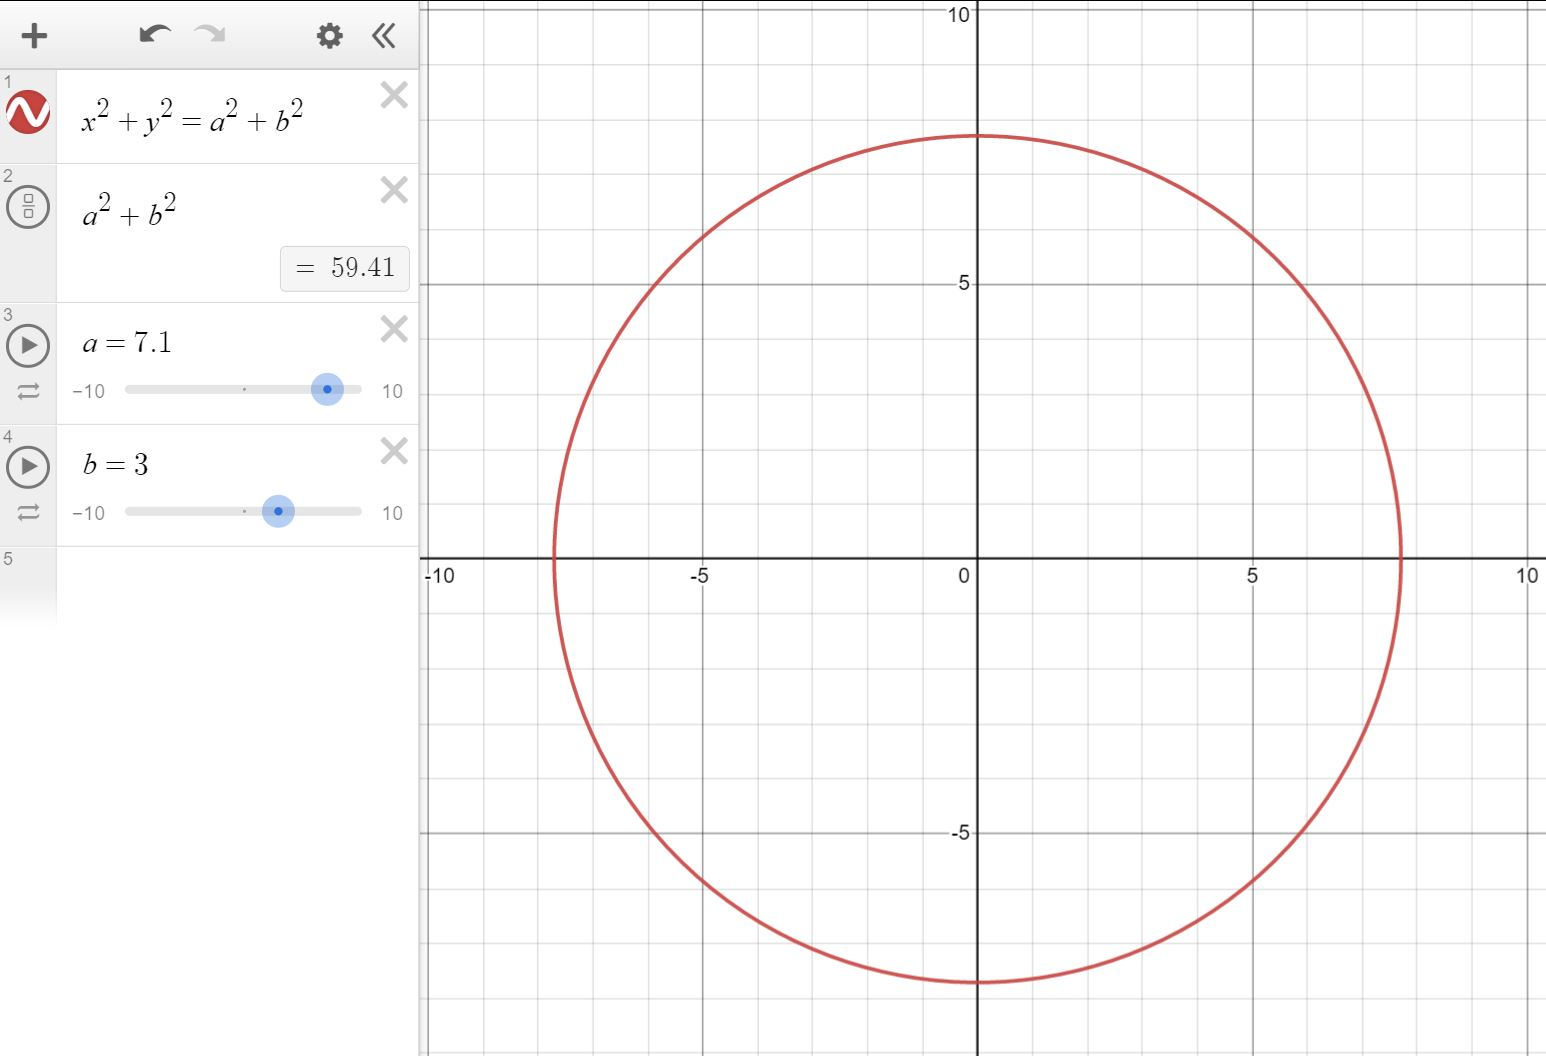
\includegraphics[width=12cm]{./pics/3.6b.jpg}}
}
\end{figure}

\newpage

\subsection{Aufgabe 3.7(H)}

\paragraph{(a)}
\begin{proof}
$ $\newline

IA: Sei $n=0$, es gilt:
\begin{equation*}
a_n=a_0=0+0+0=0\in\mathbb{N}
\end{equation*}

IV: $a_n=\frac{n}{6}+\frac{n^2}{2}+\frac{n^3}{3}$\\

IS: $\tilde{n}=n+1$\\
\begin{align*}
a_{\tilde{n}}=a_{n+1}=a_n
&=\frac{n+1}{6}+\frac{(n+1)^2}{2}+\frac{(n+1)^3}{3}\\
&=\frac{n+1}{6}+\frac{n^2+2n+1}{2}+\frac{n^3+3n^2+3n+1}{3}\\
&=\frac{n}{6}+\frac{n^2}{2}+\frac{n^3}{3}+\frac{1}{6}+\frac{2n+1}{2}+\frac{3n^2+3n+1}{3}\\
&\overset{\mathbf{IV}}{=}a_n+\frac{1}{6}+\frac{2n+1}{2}+\frac{3n^2+3n+1}{3}\\
&=a_n+\frac{6n^2+12n+6}{6}\\
&=a_n+n^2+2n+1\\
&=a_n+(n+1)^2\\
(n+1)^2\in\mathbb{N}&\Rightarrow a_n+(n+1)^2\in\mathbb{N}\\
&\Rightarrow a_{n+1}\in\mathbb{N}
\end{align*}
\end{proof}

\newpage

\paragraph{(b)}
\begin{proof}
$ $\newline

IA: Sei $n=0$, es gilt
\begin{equation*}
b_n=b_0=5^0-1=4\cdot k,\ k=0\in\mathbb{N}
\end{equation*}

IV: $b_n=5^n-1=4\cdot k,\ \exists k\in\mathbb{N}$\\

IS: $\tilde{n}=n+1$
\begin{align*}
b_{\tilde{n}}=b_{n+1}
&=5^{n+1}-1\\
&=5^n\cdot 5-1\\
&=5^n\cdot 5-1\cdot 5-4\\
&\overset{\mathbf{IV}}{=}5\cdot 4\cdot k-4\\
&=4\cdot(5\cdot k-1)\\
\exists\tilde{k}=5\cdot k-1\in\mathbb{N}&\Rightarrow b_{n+1}=4\cdot\tilde{k}\in\mathbb{N}
\end{align*}
\end{proof}

\paragraph{(c)}
\begin{proof}
$ $\newline

IA: Sei $n=0$, es gilt
\begin{equation*}
c_n=c_0=6^0-5\cdot 0+4=5=5\cdot k,\ k=1\in\mathbb{N}
\end{equation*}

IV: $c_n=6^n-5n+4=5\cdot k,\ \exists k\in\mathbb{N}$\\

IS: $\tilde{n}=n+1$
\begin{align*}
c_{\tilde{n}}=c_{n+1}
&=6^{n+1}-5(n+1)+4\\
&=6^n\cdot 6-5n-1\\
&=(6^n-5n+4+5n-4)\cdot 6-5n-1\\
&\overset{\mathbf{IV}}{=}(5\cdot k+5n-4)\cdot 6-5n-1\\
&=30k+30n-24-5n-1\\
&=5(6k+7n-5)\\
\exists\tilde{k}=6k+7n-5\in\mathbb{N}&\Rightarrow c_{n+1}=5\cdot\tilde{k}\in\mathbb{N}
\end{align*}
\end{proof}

\newpage

\subsection{Tutorium}

$M$, $N$ Mengen, $M\times N$\\
$R\subseteq M\times N$\\
Falls $\#M<\infty\wedge\#N<\infty$\\
z.B. $M=\{a,b\}$, $N=\{c,d\}$, dann $R=\{(a,c),(b,d)\}$ und $R^{-1}=\{(c,a),(d,b)\}$\\


\newpage

\section{4. Übungsblatt:}

\subsection{Aufgabe 4.1}

\paragraph{(a)}
$\begin{pmatrix}
2\\
5
\end{pmatrix}$
\begin{equation*}
\begin{pmatrix}
2\\
5
\end{pmatrix}
=\frac{2-4}{5}
\begin{pmatrix}
2\\
4
\end{pmatrix}
=-\frac{2}{5}\frac{2-3}{4}
\begin{pmatrix}
2\\
3
\end{pmatrix}
=\frac{2}{5}\frac{1}{4}\frac{2-2}{3}
\begin{pmatrix}
2\\
2
\end{pmatrix}
=0
\end{equation*}

\paragraph{(b)}
$\begin{pmatrix}
-1\\
k
\end{pmatrix}$

\begin{equation*}
\begin{pmatrix}
-1\\
0
\end{pmatrix}=1,
\begin{pmatrix}
-1\\
1
\end{pmatrix}=-1,
\begin{pmatrix}
-1\\
2
\end{pmatrix}=1,
\end{equation*}
Beh. $\begin{pmatrix}
-1\\
k
\end{pmatrix}=(-1)^k$, mit Induktion.
\begin{proof}
$ $\newline

IA:..\\

IV:..\\

IS:$\begin{pmatrix}
-1\\
k+1
\end{pmatrix}$
\begin{equation*}
\begin{pmatrix}
-1\\
k+1
\end{pmatrix}=\frac{-1-k}{k+1}
\begin{pmatrix}
-1\\
k
\end{pmatrix}=(-1)^{k+1}
\end{equation*}
\end{proof}

\paragraph{(c)}
$\begin{pmatrix}
-\frac{1}{2}\\
3
\end{pmatrix}$
\begin{equation*}
\begin{pmatrix}
-\frac{1}{2}\\
3
\end{pmatrix}
=\frac{-\frac{1}{2}-2}{3}
\begin{pmatrix}
-\frac{1}{2}\\
2
\end{pmatrix}
=-\frac{5}{6}\frac{-0.5-1}{2}
\begin{pmatrix}
-0.5\\
1
\end{pmatrix}
=\frac{5}{6}\frac{3}{4}\frac{-0.5-0}{1}
\begin{pmatrix}
-0.5\\
0
\end{pmatrix}
=-\frac{5}{16}
\end{equation*}

\newpage

\subsection{Aufgabe 4.2}

\paragraph{(a)}
z.z. $\begin{pmatrix}
x\\
k
\end{pmatrix}
=
\begin{pmatrix}
x-1\\
k-1
\end{pmatrix}\frac{x}{k}$
\begin{proof}
$ $\newline

IA: $k=1$, LS$=
\begin{pmatrix}
x\\
1
\end{pmatrix}
=\frac{x-0}{1}
\begin{pmatrix}
x\\
0
\end{pmatrix}
=\frac{x}{1}
\begin{pmatrix}
x-1\\
0
\end{pmatrix}$

IV: für $k$ gilt
\begin{equation*}
\begin{pmatrix}
x\\
k
\end{pmatrix}
=\frac{x}{k}
\begin{pmatrix}
x-1\\
k-1
\end{pmatrix}
\end{equation*}

Ziel:
\begin{equation*}
\begin{pmatrix}
x\\
k+1
\end{pmatrix}
=\frac{x}{k+1}
\begin{pmatrix}
x-1\\
k
\end{pmatrix}
\end{equation*}

IS:
\begin{align*}
\begin{pmatrix}
x\\
k+1
\end{pmatrix}
=\frac{x}{k+1}
\begin{pmatrix}
x\\
k
\end{pmatrix}
&\overset{\mathbf{IV}}{=}
\frac{x-k}{k+1}\frac{x}{k}
\begin{pmatrix}
x-1\\
k-1
\end{pmatrix}\\
&=\frac{x}{k+1}\frac{x-k}{k}\frac{k}{x-k}\frac{x-k}{k}
\begin{pmatrix}
x-1\\
k-1
\end{pmatrix}\\
&=\frac{x}{k+1}
\begin{pmatrix}
x-1\\
k
\end{pmatrix}
\end{align*}
\end{proof}

\paragraph{(b)}
z.z. $
\begin{pmatrix}
x+1\\
k
\end{pmatrix}=
\begin{pmatrix}
x\\
k-1
\end{pmatrix}+
\begin{pmatrix}
x\\
k
\end{pmatrix}
$
\begin{proof}
\begin{equation*}
\begin{pmatrix}
x+1\\
k
\end{pmatrix}
=\frac{x+1}{k}
\begin{pmatrix}
x+1-1\\
k-1
\end{pmatrix}
=\frac{x+1+k-k}{k}
\begin{pmatrix}
x\\
k-1
\end{pmatrix}
=
\underset{
\begin{pmatrix}
x\\
k
\end{pmatrix}
}{\underbrace{
\frac{\overset{x-(k-1)}{\overbrace{x+1-k}}}{k}
\begin{pmatrix}
x\\
k-1
\end{pmatrix}
}}
+
\begin{pmatrix}
x\\
k-1
\end{pmatrix}
\end{equation*}
\end{proof}

\newpage

\subsection{Aufgabe 4.3}

\begin{equation*}
x^0:=1,\ x^{n+1}=x^{n}\cdot x
\end{equation*}

\paragraph{(a)}
\begin{proof}
z.z. $x^mx^n=x^{m+n}$\\

Sei $\forall n\in\mathbb{N}_0$ fest $\rightarrow$ Induktion.\\

IA: $n=0$: $x^mx^n=x^m\cdot 1=x^m=x^{m+n}$\\

IV: $x^mx^n=x^{m+n}$\\

Ziel: $x^mx^{n+1}=x^{m+n+1}$\\

IS: LS$=x^m(x^nx)\overset{Ass.Mult}{=}(x^mx^n)x=x^{m+n}x=x^{(m+n)+1}=x^{m+(n+1)}$
\end{proof}

\paragraph{(b)}

z.z. $(x^m)^n=x^{mn}$\\

\begin{proof}
$ $\newline

Sei $\forall m\in\mathbb{N}_0$ fest\\

IA: $n=0$,: $(x^m)^0=1=x^0=x^{m\cdot 0}$\\

IV: $(x^m)^n=x^{mn}$\\

Ziel: $(x^m)^{n+1}=x^{m(n+1)}$\\

IS: $(x^m)^{n+1}=(x^m)^n\cdot x^m\overset{\mathbf{IV}}{=}x^{mn}x^n\overset{(a)}{=}x^{mn+n}$\\
\end{proof}

\paragraph{(c)}
\begin{proof}
$ $\newline

IA: $n=0$ $\rightarrow$ $(x\cdot y)^n=1=1\cdot 1=x^0y^0$\\

IV: ......\\

IS: $(xy)^{n+1}=(xy)^n(xy)\overset{\mathbf{IV}}{=}(x^ny^n)(xy)\overset{Field-Axiom}{=}(x^nx)(y^ny)=x^{n+1}y^{n+1}$
\end{proof}


\newpage

\subsection{Aufgabe 4.4}
See definition of Group, Monoid etc.

\newpage

\subsection{Aufgabe 4.5}

Inverse: Sei $(G,\cdot)$ Gruppe\\
Man sagte dass $f\in G$ ist Inverse von $g\in G$\\
$\overset{Def}{\Leftrightarrow}$ $f\cdot g=g\cdot f=e$, Notation: $f=:g^{-1}$

\paragraph{(a)}
\begin{proof}
$ $\newline

z.z. $(a^{-1})^{-1}=a$ falls $a\neq 0$\\

$\Leftrightarrow$ $a$ ist Inv. von $a^{-1}$ $\Leftrightarrow$ $a\cdot a^{-1}=a^{-1}\cdot a=e$\\

Das gilt da $a$ Inv. von $a^{-1}$
\end{proof}

\paragraph{(b)}
\begin{proof}
$ $\newline

z.z. $(ab)^{-1}=a^{-1}b^{-1}$\\

$(ab)(a^{-1}b^{-1})\overset{F.Axiom}{=}(a\cdot a^{-1})(b\cdot b^{-1})=1$\\

$(a^{-1}b^{-1})(ab)\overset{F.Axiom}{=}(a^{-1}\cdot a)(b^{-1}\cdot b)=1$\\
\end{proof}

\newpage

\subsection{Aufgabe 4.6(H)}

\paragraph{(a)}
\begin{proof}
$ $\newline

z.z. $\forall n\in\mathbb{N}_{\geq1}$, es gilt
\begin{equation*}
\sum_{k=0}^{n}\frac{(-1)^k}{k+1}
\begin{pmatrix}
n \\
k
\end{pmatrix}
=
\frac{1}{n+1}
\end{equation*}

Wir haben
\begin{align*}
\begin{pmatrix}
n \\
k
\end{pmatrix}
&=
\frac{n}{k}
\begin{pmatrix}
n-1 \\
k-1
\end{pmatrix}\\
\begin{pmatrix}
n+1 \\
k+1
\end{pmatrix}
&=
\frac{n+1}{k+1}
\begin{pmatrix}
n \\
k
\end{pmatrix}\\
\frac{1}{n+1}
\begin{pmatrix}
n+1 \\
k+1
\end{pmatrix}
&=
\frac{1}{k+1}
\begin{pmatrix}
n \\
k
\end{pmatrix}
\end{align*}

betrachten
\begin{align*}
\sum_{k=0}^{n}\frac{(-1)^k}{n+1}
\begin{pmatrix}
n+1 \\
k+1
\end{pmatrix}
&=
\frac{1}{n+1}\\
\frac{1}{n+1}
\sum_{k=0}^{n}(-1)^k
\begin{pmatrix}
n+1 \\
k+1
\end{pmatrix}
&=
\frac{1}{n+1}\\
\end{align*}

dann, z.z. $\forall n\in\mathbb{N}_{\geq1}$
\begin{equation*}
\sum_{k=0}^{n}(-1)^k
\begin{pmatrix}
n+1 \\
k+1
\end{pmatrix}
=
1
\end{equation*}

IA: Sei $n=1$, es gilt
\begin{equation*}
\sum_{k=0}^{1}(-1)^k
\begin{pmatrix}
1+1 \\
k+1
\end{pmatrix}
=
1
\begin{pmatrix}
2 \\
1
\end{pmatrix}+
(-1)
\begin{pmatrix}
2 \\
2
\end{pmatrix}
=
2-1
=
1
\end{equation*}

IV: $\forall n\in\mathbb{N}_{\geq1}$, es gilt
\begin{equation*}
\sum_{k=0}^{n}(-1)^k
\begin{pmatrix}
n+1 \\
k+1
\end{pmatrix}
=
1
\end{equation*}

IS: Sei $\tilde{n}=n+1$, wir betrachten
\begin{align*}
\sum_{k=0}^{\tilde{n}}(-1)^k
\begin{pmatrix}
\tilde{n}+1 \\
k+1
\end{pmatrix}
&=
\sum_{k=0}^{n+1}(-1)^k
\begin{pmatrix}
n+2 \\
k+1
\end{pmatrix}\\
&=
\sum_{k=0}^{n+1}(-1)^k
\begin{pmatrix}
n+1 \\
k+1
\end{pmatrix}+
\sum_{k=0}^{n+1}(-1)^k
\begin{pmatrix}
n+1 \\
k
\end{pmatrix}\\
&=
\sum_{k=0}^{n}(-1)^k
\begin{pmatrix}
n+1 \\
k+1
\end{pmatrix}+
(-1)^{n+1}
\begin{pmatrix}
n+1 \\
n+2
\end{pmatrix}+
\sum_{k=0}^{n}(-1)^k
\begin{pmatrix}
n+1 \\
k
\end{pmatrix}+
(-1)^{n+1}
\begin{pmatrix}
n+1 \\
n+1
\end{pmatrix}\\
&\overset{\mathbf{IV}}{=}
1+0+
\sum_{k=0}^{n}(-1)^k
\begin{pmatrix}
n+1 \\
k
\end{pmatrix}+
(-1)^{n+1}\\
&=1+0+0=1
\end{align*}
\end{proof}

\newpage

\paragraph{(b)}
$ $\newline

Vermutung: $\forall n\in\mathbb{N}_{\geq1}$ und $m\in\mathbb{N}_{\geq 1}$
\begin{equation*}
\sum_{k=1}^{n}\prod_{i=0}^{m-1}(k+i)=\frac{1}{m+1}\prod_{i=0}^{m}(n+i)
\end{equation*}
\begin{proof}
$ $\newline

IA: Sei $n=1$, es gilt
\begin{equation*}
\sum_{k=1}^{1}\prod_{i=0}^{m-1}(k+i)=\prod_{i=0}^{m-1}(1+i)=\frac{1}{1+m}\prod_{i=0}^{m}(1+i)
\end{equation*}

IV: $\forall n\in\mathbb{N}_{\geq1}$ und $m\in\mathbb{N}_{\geq 1}$
\begin{equation*}
\sum_{k=1}^{n}\prod_{i=0}^{m-1}(k+i)=\frac{1}{m+1}\prod_{i=0}^{m}(n+i)
\end{equation*}

IS: Sei $\tilde{n}=n+1$, wir betrachten
\begin{align*}
\sum_{k=1}^{\tilde{n}}\prod_{i=0}^{m-1}(k+i)
&=
\sum_{k=1}^{n+1}\prod_{i=0}^{m-1}(k+i)\\
&=
\sum_{k=1}^{n}\prod_{i=0}^{m-1}(k+i)+
\prod_{i=0}^{m-1}(n+1+i)\\
&\overset{\mathbf{IV}}{=}
\frac{1}{m+1}\prod_{i=0}^{m}(n+i)+
\prod_{i=0}^{m-1}(n+1+i)\\
&=
\frac{1}{m+1}\prod_{i=0}^{m}(n+i)+
\frac{1}{n}\prod_{i=0}^{m}(n+i)\\
&=
\Big(\frac{1}{m+1}+\frac{1}{n}\Big)\prod_{i=0}^{m}(n+i)\\
&=
\frac{n+m+1}{n(m+1)}\prod_{i=0}^{m}(n+i)\\
&=
\frac{1}{m+1}\frac{n+m+1}{n}\prod_{i=0}^{m}(n+i)\\
&=
\frac{1}{m+1}\prod_{i=0}^{m}(n+1+i)
\end{align*}
\end{proof}

\newpage

\subsection{Aufgabe 4.7(H)}
\begin{proof}
$ $\newline

IA: Sei $n=0$, es gilt
\begin{equation*}
\sum_{k=0}^{0}(-1)^k\cdot
\begin{pmatrix}
x \\
k
\end{pmatrix}
=
(-1)^0\cdot
\begin{pmatrix}
x \\
0
\end{pmatrix}
=
1
=
(-1)^0\cdot
\begin{pmatrix}
x-1 \\
0
\end{pmatrix}
\end{equation*}

IV: $x\in\mathbb{R}$, $n\in\mathbb{N}$
\begin{equation*}
\sum_{k=0}^{n}(-1)^k\cdot
\begin{pmatrix}
x \\
k
\end{pmatrix}
=
(-1)^n\cdot
\begin{pmatrix}
x-1 \\
n
\end{pmatrix}
\end{equation*}

IS: Sei $\tilde{n}=n+1$, wir betrachten
\begin{align*}
\sum_{k=0}^{\tilde{n}}(-1)^k\cdot
\begin{pmatrix}
x \\
k
\end{pmatrix}
&=
\sum_{k=0}^{n+1}(-1)^k\cdot
\begin{pmatrix}
x \\
k
\end{pmatrix}\\
&=
\sum_{k=0}^{n}(-1)^k\cdot
\begin{pmatrix}
x \\
k
\end{pmatrix}+
(-1)^{n+1}\cdot
\begin{pmatrix}
x \\
n+1
\end{pmatrix}\\
&\overset{\mathbf{IV}}{=}
(-1)^n\cdot
\begin{pmatrix}
x-1 \\
n
\end{pmatrix}+
(-1)^{n+1}\cdot
\begin{pmatrix}
x \\
n+1
\end{pmatrix}\\
&=
-(-1)^{n+1}\cdot
\begin{pmatrix}
x-1 \\
n
\end{pmatrix}+
(-1)^{n+1}\cdot
\begin{pmatrix}
x \\
n+1
\end{pmatrix}\\
&=
(-1)^{n+1}\cdot\Bigg(
\begin{pmatrix}
x \\
n+1
\end{pmatrix}-
\begin{pmatrix}
x-1 \\
n
\end{pmatrix}
\Bigg)\\
&=
(-1)^{n+1}\cdot\Bigg(
\begin{pmatrix}
x-1 \\
n+1
\end{pmatrix}+
\begin{pmatrix}
x-1 \\
n
\end{pmatrix}-
\begin{pmatrix}
x-1 \\
n
\end{pmatrix}
\Bigg)\\
&=
(-1)^{n+1}\cdot
\begin{pmatrix}
x-1 \\
n+1
\end{pmatrix}
\end{align*}
\end{proof}

\newpage

\subsection{Tutorium}

\textsc{Gauss Klammern} oder \textsc{Floor and Ceiling Function}\\

$\forall x,y\in\mathbb{R}$, $x-y\in\mathbb{Z}$\\

$\Rightarrow$ $x-\lfloor x\rfloor=y-\lfloor y\rfloor$\\

"$\Leftarrow$" $x-y=\lfloor x\rfloor-\lfloor y\rfloor$\\

$\Rightarrow$ $x-y\in\mathbb{Z}$\\

"$\Rightarrow$" $x-y\in\mathbb{Z}$\\

$\Leftrightarrow$ $\exists k\in\mathbb{Z}$: $x-y=k$\\

$\Rightarrow$ $x-\lfloor x\rfloor-(y-\lfloor y\rfloor)=$\\


\newpage

\section{5. Übungsblatt:}

\subsection{Aufgabe 5.1}

$n^{n+1}
\begin{pmatrix}
= \\
< \\
>
\end{pmatrix}
(n+1)^n$\\

$n=3$, $LS=3^4=81$ $RS=4^3=64$\\

Vermutung: $n^{n+1}>(n+1)^n$\\

\begin{equation*}
\Leftrightarrow1>\frac{(n+1)^n}{n^{n+1}}=\frac{1}{n}(1+\frac{1}{n})^n
\end{equation*}
\begin{align*}
&=\frac{1}{n}\Bigg(\sum_{k=0}^n
\begin{pmatrix}
n \\
k
\end{pmatrix}
1^{n-k}
(\frac{1}{n})^k
\Bigg)\\
&=\frac{1}{n}\Bigg(\sum_{k=0}^n\frac{n!}{(n-k)!k!}\frac{1}{n^k}\Bigg)\\
(n-k)!\mbox{ hat }k\mbox{ Faktoren}&=\frac{1}{n}\Bigg(\sum_{k=0}^n
\underset{\leq 1}{\underbrace{\prod_{i=1}^k\frac{n-k+i}{n}}}\cdot\frac{1}{k!}\Bigg)\\
&\leq\frac{1}{n}\Bigg(\sum_{k=0}^n\frac{1}{k!}\Bigg)\\
&=\frac{1}{n}\Bigg(\frac{5}{2}+\underset{\leq\frac{n-2}{6}}{\underbrace{\sum_{k=3}^n\underset{\leq\frac{1}{6}}{\underbrace{\frac{1}{k!}}}}}\Bigg)\\
&\leq\frac{1}{6}+\frac{13}{6n}\\
n\in\mathbb{N}_{>3}&=\frac{1}{6}+\frac{13}{18}=\frac{16}{18}<1
\end{align*}

\newpage

\subsection{Aufgabe 5.2}

$\frac{a}{b}=a\cdot b^{-1}$ mit $b\neq a$

\paragraph{(a)}

\subparagraph{(i)}
\begin{proof}
$ $\newline

z.z. $\frac{a}{b}\cdot\frac{c}{d}=\frac{ac}{bd}$\\
\begin{align*}
&(a\cdot b^{-1})\cdot(c\cdot d^{-1})\\
&a\cdot(b^{-1}(c\cdot d^{-1}))\\
&a(b^{-1}(d^{-1}\cdot c))\\
&a((b^{-1}\cdot d^{-1})\cdot c)\\
&a(c\cdot(b^{-1}\cdot d^{-1}))\\
&(a\cdot c)\cdot(b^{-1}\cdot d^{-1})\\
&(a\cdot c)\cdot(b\cdot d)^{-1}
\end{align*}
\end{proof}

\subparagraph{(ii)}
\begin{proof}
$ $\newline

$\frac{\frac{a}{b}}{\frac{c}{d}}$\\

\begin{align*}
LS=\frac{(a\cdot b^{-1})}{c\cdot d^{-1}}&=(a\cdot b^{-1})((c\cdot d^{-1})^{-1})\\
&=(a\cdot b^{-1})(c^{-1}\cdot d)\\
&=a\cdot(b^{-1}\cdot c^{-1})\cdot d\\
&=a\cdot d\cdot(b^{-1}\cdot c^{-1})\\
&=\ldots
\end{align*}
\end{proof}

\paragraph{(b)}
$ $\newline

\href{https://en.wikipedia.org/wiki/Field_(mathematics)#Classic_definition}{Field axioms}\\

\url{https://en.wikipedia.org/wiki/Field_(mathematics)#Classic_definition}

\newpage

\paragraph{(c)}

\newpage

\subsection{Aufgabe 5.3}

\newpage

\subsection{Aufgabe 5.4}

\paragraph{(a)}
$|x-a|<\epsilon$ $\Leftrightarrow$ $x\in(a-\epsilon,a+\epsilon)$\\

dann $x\geq a$ oder $x<a$

\paragraph{(b)}

\paragraph{(c)}
$\frac{1}{x}<\frac{1}{x+1}$\\

falls $x>0$, dann $x+1<x$\\

$((x+1)+x)\frac{1}{x}<(x+1)x\frac{1}{x+1}$\\

dann $x+1<x$ $contradiction$ denn $\forall x\in\mathbb{R}$, $x+1>x$

!!!!!!3 Falle.

\subsection{Aufgabe 5.5}

\newpage

\subsection{Aufgabe 5.6(H)}

\paragraph{(a)}
\begin{proof}
$ $\newline

z.z. $\frac{ad}{bd}=\frac{a}{b}$
\begin{align*}
\frac{ad}{bd}
&=(ad)(bd)^{-1}\\
&=(ad)(b^{-1}d^{-1})\\
&=a(d(b^{-1}d^{-1}))\\
&=a(d(d^{-1}b^{-1}))\\
&=a((dd^{-1})b^{-1})\\
&=ab^{-1}\\
&=\frac{a}{b}
\end{align*}
\end{proof}

\paragraph{(b)}
\begin{proof}
$ $\newline

z.z. $\frac{a}{b}+\frac{c}{d}=\frac{ad+bc}{bd}$
\begin{align*}
\frac{ad+bc}{bd}
&=(ad+bc)(bd)^{-1}\\
&=(ad)(bd)^{-1}+(bc)(bd)^{-1}\\
&=(ad)(b^{-1}d^{-1})+(bc)(b^{-1}d^{-1})\\
&=(ad)(d^{-1}b^{-1})+(cb)(b^{-1}d^{-1})\\
&=a(d(d^{-1}b^{-1}))+c(b(b^{-1}d^{-1}))\\
&=a((dd^{-1})b^{-1})+c((bb^{-1})d^{-1})\\
&=ab^{-1}+cd^{-1}\\
&=\frac{a}{b}+\frac{c}{d}
\end{align*}
\end{proof}

\newpage

\subsection{Aufgabe 5.7(H)}

$Ohne\ weitere\ Meldung\ sei\ x\in\mathbb{R}$

\paragraph{(a)}
$ $\newline

Wenn $x-3>0$, daraus folgt $x>3$ und $x+1>0$, dann
\begin{align*}
\frac{2}{x+1}&<\frac{1}{x-3}\\
2(x-3)&<x+1\\
x&<7\hspace{1em}widerspruchsfrei\\
\Rightarrow\hspace{1em}3<x&<7
\end{align*}

Wenn $x-3<0$ und $x+1>0$, daraus folgt $-1<x<3$, dann
\begin{align*}
\frac{2}{x+1}&<\frac{1}{x-3}\\
2(x-3)&>x+1\\
x&>7\hspace{1em}\lightning
\end{align*}

Wenn $x+1<0$, daraus folgt $x<-1$ und $x-3<0$, dann
\begin{align*}
\frac{2}{x+1}&<\frac{1}{x-3}\\
2(x-3)&<x+1\\
x&<7\hspace{1em}widerspruchsfrei\\
\Rightarrow\hspace{1em}x&<-1
\end{align*}

$Folgerung:$ $(x<-1)\vee(3<x<7)$

\paragraph{(b)}
$ $\newline

Wenn $x-3\geq0$, daraus folgt $x\geq3$ und $x+1>0$, dann
\begin{align*}
|x+1|+|x-3|&<6\\
x+1+x-3&<6\\
x&<4\hspace{1em}widerspruchsfrei\\
\Rightarrow\hspace{1em}3\leq x&<4
\end{align*}

Wenn $x-3<0$ und $x+1\geq0$, daraus folgt $-1\leq x<3$, dann
\begin{align*}
|x+1|+|x-3|&<6\\
x+1+3-x&<6\\
4&<6\hspace{1em}widerspruchsfrei\\
\Rightarrow\hspace{1em}-1\leq x&<3
\end{align*}

Wenn $x+1<0$, daraus folgt $x<-1$ und $x-3<0$, dann
\begin{align*}
|x+1|+|x-3|&<6\\
-x-1+3-x&<6\\
-2&<x\hspace{1em}widerspruchsfrei\\
\Rightarrow\hspace{1em}-2<x&<-1
\end{align*}

$Folgerung:$ $-2<x<4$

\newpage

\paragraph{(c)}
$ $\newline

Wenn $|x+3|>1$, $||x+3|-1|=|x+3|-1$, daraus folgt $-2\leq x$ oder $x\leq -4$\\

$-2\leq x$:

$||x+3|-1|=|x+3|-1=x+3-1=x+2=2$ folgt $x=0$ $widerspruchsfrei$\\

$x\leq -4$:

$||x+3|-1|=|x+3|-1=-x-3-1=-x-4=2$ folgt $x=-6$ $widerspruchsfrei$\\

Wenn $|x+3|<1$, $||x+3|-1|=1-|x+3|$, daraus folgt $-4<x<-2$\\

$-4<x<-3$:

$||x+3|-1|=1-|x+3|=1+x+3=x+4=2$ folgt $x=-2$ $\lightning$\\

$-3\leq x<-2$:

$||x+3|-1|=1-|x+3|=1-x-3=-x-2=2$ folgt $x=-4$ $\lightning$\\

$Folgerung:$ $(x=0)\vee(x=-6)$


\newpage

\section{6. Übungsblatt:}

\subsection{Aufgabe 6.1}

\subsection{Aufgabe 6.2}

\subsection{Aufgabe 6.3}

\subsection{Aufgabe 6.4}

\newpage

\subsection{Aufgabe 6.5(H)}

\paragraph{(a)}
\begin{align*}
\frac{2n+1}{3n}+\frac{3n}{2n-1}
&=\frac{2}{3}+\frac{1}{3n}+\frac{3n}{2n-1}\\
&=\frac{2}{3}+\frac{1}{3n}+\frac{3n}{n(2-\frac{1}{n})}\\
&=\frac{2}{3}+\frac{1}{3n}+\frac{3}{2-\frac{1}{n}}\\
\mbox{offenbar}\lim_{n\rightarrow\infty}\Bigg(\frac{2}{3}+\frac{1}{3n}+\frac{3}{2-\frac{1}{n}}\Bigg)&=\frac{2}{3}+\frac{3}{2}=\frac{13}{6}
\end{align*}

\paragraph{(b)}
\begin{align*}
\begin{pmatrix}
2n \\
n
\end{pmatrix}
&=\frac{(2n)!}{n!n!}\\
&=\frac{\prod_{k=1}^{2n}k}{\prod_{k=1}^{n}k\cdot\prod_{k=1}^{n}k}\\
&=\frac{\prod_{k=n+1}^{2n}k}{\prod_{k=1}^{n}k}
\end{align*}
\begin{align*}
\frac{a_{n+1}}{n}=\frac{\prod_{k=n+2}^{2n+2}k}{\prod_{k=1}^{n+1}k}\frac{\prod_{k=1}^{n}k}{\prod_{k=n+1}^{2n}k}
&=\frac{(2n+1)(2n+2)}{(n+1)^2}\\
&=\frac{4n^2+5n+2}{n^2+2n+1}\\
&=\frac{4+\frac{5}{n}+\frac{2}{n^2}}{1+\frac{2}{n}+\frac{1}{n^2}}\\
\mbox{offenbar}\lim_{n\rightarrow\infty}\Bigg|\frac{4+\frac{5}{n}+\frac{2}{n^2}}{1+\frac{2}{n}+\frac{1}{n^2}}\Bigg|&=4>0\\
&\Rightarrow
\begin{pmatrix}
2n \\
n
\end{pmatrix}\mbox{divergent}
\end{align*}

\subsection{Aufgabe 6.6(H)}

\paragraph{(a)}
$ $\newline
Sei $a_n=0$, dann $\lim_{n\rightarrow\infty}a_n=0$ mit $\frac{a_n}{b_n}=0$, dann $\lim_{n\rightarrow\infty}(\frac{a_n}{b_n})_{n\in\mathbb{N}}=0$ für beliebige $b_n$ inkl. Nullfolge. $\lightning$

\paragraph{(b)}
\begin{proof}
Sei $\lim_{n\rightarrow\infty}b_n=0$, dann $\lim_{n\rightarrow\infty}\frac{1}{b_n}=\infty$ folgt $\frac{1}{b_n}$ divergent.
\end{proof}

\paragraph{(c)}
$ $\newline
Sei $a_n=0$, dann $\lim_{n\rightarrow\infty}a_n=0$ mit $(a_n\cdot b_n)=0$ , dann $\lim_{n\rightarrow\infty}(a_n\cdot b_n)=0$ für beliebige $b_n$ inkl. divg. Folge. $\lightning$


\newpage

\section{7. Übungsblatt}

\subsection{Aufgabe 7.1}

\subsection{Aufgabe 7.2}

\subsection{Aufgabe 7.3}

\subsection{Aufgabe 7.4}

\subsection{Aufgabe 7.5}

\newpage

\subsection{Aufgabe 7.6(H)}

Wir beweisen zuerst die folgende Gleichung
\begin{equation*}
\underset{\geq\sqrt{a}}{\underbrace{(\sqrt{a_n}+\sqrt{a})}}\cdot|\sqrt{a_n}-\sqrt{a}|=|a_n-a|
\end{equation*}
\begin{proof}
\begin{equation*}
(\sqrt{a_n}+\sqrt{a})\cdot|\sqrt{a_n}-\sqrt{a}|=\left\{\begin{array}{lcl}
(\sqrt{a_n}>\sqrt{a}) & (\sqrt{a_n}+\sqrt{a})\cdot(\sqrt{a_n}-\sqrt{a})=(a_n-a)=|a_n-a|\\
(\sqrt{a_n}<\sqrt{a}) & (\sqrt{a_n}+\sqrt{a})\cdot(\sqrt{a}-\sqrt{a_n})=-(a_n-a)=|a_n-a|
\end{array}\right.
\end{equation*}

$a_n\geq0$ $\Leftrightarrow$ $\sqrt{a_n}\geq0$

$\sqrt{a_n}\geq0$ $\Leftrightarrow$ $\sqrt{a_n}+\sqrt{a}\geq\sqrt{a}$

\end{proof}

Sei $\lim_{n\rightarrow\infty}a_n=a$

$\Leftrightarrow$ $\forall\varepsilon\in\mathbb{R}_{>0}$, $\exists N\in\mathbb{N}$, $\forall n\in\mathbb{N}_{>N}$, $|a_n-a|<\varepsilon$\\

dann

\begin{align*}
(\sqrt{a_n}+\sqrt{a})\cdot|\sqrt{a_n}-\sqrt{a}|&=|a_n-a|\\
|\sqrt{a_n}-\sqrt{a}|&=\frac{|a_n-a|}{(\sqrt{a_n}+\sqrt{a})}<\frac{\varepsilon}{\sqrt{a}}
\end{align*}

Sei $\tilde{\varepsilon}=\frac{\varepsilon}{\sqrt{a}}\in\mathbb{R}_{>0}$, dann $|\sqrt{a_n}-\sqrt{a}|<\tilde{\varepsilon}$

$\Leftrightarrow$ $\lim_{n\rightarrow\infty}\sqrt{a_n}=\sqrt{a}$

\newpage

\subsection{Aufgabe 7.7(H)}
$ $\newline

Wir beweisen nun mittels Vollständige Induktion, dass $a_n$ monoton wachsend ist.
\begin{proof}
$ $\newline

Sei $a_{n+1}=\sqrt{c+a_n}$\\

IA:

Sei $n=1$, dann gilt
\begin{align*}
\frac{a_2}{a_1}&=\frac{\sqrt{c+\sqrt{c}}}{\sqrt{c}}\\
\frac{a_2^2}{a_1^2}&=\frac{c+\sqrt{c}}{c}\overset{(c>0)}{>}1\\
\overset{(c>0)}{\Leftrightarrow}\frac{a_2}{a_1}&>1
\end{align*}\\

IV:

\begin{equation*}
\frac{a_{n+1}}{a_n}>1\hspace{1em}\Leftrightarrow\hspace{1em}\frac{\sqrt{c+a_n}}{a_n}>1
\end{equation*}\\

IS:

Wir setzen $\tilde{n}=n+1$ ein,
\begin{align*}
\frac{a_{\tilde{n}+1}}{a_{\tilde{n}}}=\frac{a_{(n+1)+1}}{a_{n+1}}
&=\frac{\sqrt{c+a_{n+1}}}{\sqrt{c+a_n}}\\
\frac{(a_{(n+1)+1})^2}{a_{n+1}^2}
&=\frac{c+\sqrt{c+a_n}}{c+a_n}\overunderset{\mathbf{IV}}{(c>0)}{>}1\\
\overset{(c>0)}{\Leftrightarrow}\frac{a_{\tilde{n}+1}}{a_{\tilde{n}}}&>1
\end{align*}
\end{proof}

\newpage

Wir beweisen nun, dass $a_n$ von oben beschränkt ist.
\begin{proof}
\begin{align*}
a_{n+1}&=\sqrt{c+a_n}\\
a_n&=\sqrt{c+a_{n-1}}\\
\Rightarrow\lim_{n\rightarrow\infty}a_n&=\sqrt{\lim_{n\rightarrow\infty}(c+a_{n-1})}\\
&=\sqrt{c+\lim_{n\rightarrow\infty}a_{n-1}}
\end{align*}

Sei $\lim_{n\rightarrow\infty}a_n=a=\lim_{n\rightarrow\infty}a_{n-1}$, dann
\begin{align*}
a&=\sqrt{c+a}\\
a^2&=c+a\\
a^2-a-c&=0\\
\Leftrightarrow a&=\left\{\begin{array}{lcl}
\frac{1+\sqrt{1+4c}}{2}\overset{(c>0)}{>}1 \\
\frac{1-\sqrt{1+4c}}{2}\overset{(c>0)}{<}0
\end{array}\right.
\end{align*}
Wir haben schon gezeigt, dass $a_n>0$ monoton wachsend ist, dann  muss $a>0$ sein. Deshalb haben wir $a=\frac{1+\sqrt{1+4c}}{2}$. Dann ist $\lim_{n\rightarrow\infty}a_n=a=\frac{1+\sqrt{1+4c}}{2}$

\end{proof}


\newpage

\section{8. Übungsblatt}

\subsection{Aufgabe 8.1}

\begin{proof}
$ $\newline

\end{proof}

\subsection{Aufgabe 8.2}

c) geo. Reihe mit

\newpage

\subsection{Aufgabe 8.3}
$ $\newline

Maj. Krit. : Seien $(a_n)_n,(b_n)_n\subseteq\mathbb{R}$, $\forall n\in\mathbb{N}$: $b_n>0$

Falls $\exists N\in\mathbb{N}$, $\exists c\in\mathbb{R}$, $\forall n\in\mathbb{N}_{>N}$: $|a_n|\leq c\cdot b_n$

und falls $\sum_{1}^{\infty}b_n$ konv. dann konv. $\sum_{1}^{\infty}$ abs.

\begin{proof}
$ $\newline

$(a_n)_n\in\mathbb{R}$ und $\exists\theta\in(0,1)$ und $\exists N\in\mathbb{N}$

sodass: $\forall n\geq N$ gilt $\sqrt[n]{|a_n|}<\theta$

da $\sum_{n=1}^{\infty}\theta^n$ konv. (geom. Reihe) $\Leftrightarrow$ $|a_n|<\theta^n$

nach Maj. Krit. konv. $\sum a_n$ abs.
\end{proof}

\newpage

\subsection{Aufgabe 8.4}

\paragraph{(a)}
$ $\newline

$a_n=\frac{n!}{n^n}$

Quotient-Krit.

\begin{align*}
\Big|\frac{a_{n+1}}{a_n}\Big|
&=\Big|\frac{(n+1)!}{(n+1)^{n+1}}\Big|\\
&=\Big|\frac{n^n}{(n+1)^n}\Big|\\
()^{-1}&=\underset{(n\rightarrow0)\rightarrow e}{\underbrace{\Bigg(\Big(\frac{n+1}{n}\Big)^n\Bigg)^{-1}}}
\end{align*}

$e^x:=\lim_{n\rightarrow\infty}(1+\frac{x}{n})^n$

$\Rightarrow$ $|\frac{a_{n+1}}{a_n}|=((1+\frac{1}{n})^n)^{-1}\overset{n\rightarrow\infty}{\longrightarrow}e^{-1}$\\

Sei nun $\tilde{\epsilon}=1-e^{-1}$ dann: $\underset{\theta}{\underbrace{e^{-1}+\frac{\tilde{\epsilon}}{2}}}<1$

$e^{-1}+\frac{\tilde{\epsilon}}{2}=e^{-1}+\frac{1-e^{-1}}{2}=\frac{1+e^{-1}}{2}<1$

dann $\lim_{n\rightarrow\infty}|\frac{a_{n+1}}{a_n}|=e^{-1}$ for $\epsilon_i=\frac{\tilde{\epsilon}}{2}$ $\exists N\in\mathbb{N}$ sind

$\forall n\in\mathbb{N}_{>N}$: $|\frac{a_{n+1}}{a_n}-e^{-1}|<\frac{\tilde{\epsilon}}{2}$

$\Rightarrow$ $\frac{a_{n+1}}{a_n}<e^{-1}+\frac{\tilde{\epsilon}}{2}$

\paragraph{(b)}
$ $\newline

$a_n=(\sqrt[n]{n}-1)^n$

dann $\sqrt[n]{|a_n|}=\sqrt[n]{(\sqrt[n]{n}-1)^n}=\sqrt[n]{n}-1\overset{n\rightarrow\infty}{\longrightarrow}0$

z.B. Sei $\theta_i=\frac{1}{2}=\epsilon$ $\exists N\in\mathbb{N}$

$\forall n\in\mathbb{N}_{>N}$: $|\sqrt[n]{n}-1-0|<\epsilon=\frac{1}{2}$ $\Rightarrow$ $\sqrt[n]{n}-1<\frac{1}{2}$

\paragraph{(c)}
$ $\newline

$a_n=(-1)^n\frac{n+1}{n}$

$a_n$ kein Nullfolge

nicht konv.

\paragraph{(d)}
$ $\newline

$a_N=\frac{n+4}{n^3-3n+1}$

mit Harmonische Reihe ($n>1$ konv.)

\begin{align*}
&=\frac{n}{n^3-3n+1}+\frac{4}{n^3-3n+1}\\
&\leq\frac{n}{n^3-3n}+\frac{4}{n^3-3n}\\
&=\frac{1}{n^2-3}+\frac{4}{n^3-3n}\\
&\leq\frac{1}{(n-3)^2}+\frac{1}{(n-4)^3}\hspace{1em}for\hspace{1em}n>20
\end{align*}

\newpage

\paragraph{(e)}
\begin{align*}
a_n
&=\ldots\\
&=\frac{2\sqrt{n}}{n-1}\\
&\geq\frac{2\sqrt{n}}{n}=\frac{2}{\sqrt{n}}\ div.
\end{align*}

\paragraph{(f)}
$ $\newline

\newpage

\subsection{Aufgabe 8.5(H)}

\paragraph{(a)}
$ $\newline

For
\begin{equation*}
\sum_{n=1}^{\infty}a_n=\sum_{n=1}^{\infty}\frac{n^2}{2^n}
\end{equation*}

We determine with ratio test:
\begin{align*}
\frac{a_{n+1}}{a_n}
&=\frac{(n+1)^2}{2^{n+1}}\frac{2^n}{n^2}\\
&=\frac{n^2+2n+1}{2n^2}\\
&=\frac{1}{2}+\frac{1}{n}+\frac{1}{2n^2}\\
&\mbox{for }n\rightarrow\infty\mbox{ we have}\\
\lim_{n\rightarrow\infty}\Bigg|\frac{a_{n+1}}{a_n}\Bigg|&=\frac{1}{2}<1\\
&\Rightarrow\mbox{this series is convergent}
\end{align*}

\paragraph{(b)}
$ $\newline

For
\begin{equation*}
\sum_{n=1}^{\infty}a_n=\sum_{n=1}^{\infty}\Big(1+\frac{1}{n^2}\Big)^n
\end{equation*}

We determine with ratio test:
\begin{align*}
\frac{a_{n+1}}{a_n}
&=\frac{(1+\frac{1}{(n+1)^2})^{n+1}}{(1+\frac{1}{n^2})^n}\\
&=\frac{\Big((1+\frac{1}{(n+1)^2})^{(n+1)^2}\Big)^{\frac{1}{n+1}}}{\Big((1+\frac{1}{n^2})^{n^2}\Big)^\frac{1}{n}}\\
(\mbox{substitute }\tilde{n}=n^2,\tilde{n}'=(n+1)^2)&=
\frac{\Big((1+\frac{1}{\tilde{n}'})^{\tilde{n}'}\Big)^{\frac{1}{n+1}}}{\Big((1+\frac{1}{\tilde{n}})^{\tilde{n}}\Big)^\frac{1}{n}}
\end{align*}

with $n\rightarrow\infty$, we have
\begin{equation*}
\lim_{n\rightarrow\infty}\tilde{n}=\lim_{n\rightarrow\infty}\tilde{n}'=\lim_{n\rightarrow\infty}n=\infty,\hspace{1em}\lim_{n\rightarrow\infty}\frac{1}{n+1}=\lim_{n\rightarrow\infty}\frac{1}{n}=0
\end{equation*}

therefore
\begin{equation*}
\lim_{n\rightarrow\infty}\Bigg|\frac{a_{n+1}}{a_n}\Bigg|
\lim_{n\rightarrow\infty}\Bigg|\frac{\Big((1+\frac{1}{\tilde{n}'})^{\tilde{n}'}\Big)^{\frac{1}{n+1}}}{\Big((1+\frac{1}{\tilde{n}})^{\tilde{n}}\Big)^\frac{1}{n}}\Bigg|=\lim_{n\rightarrow\infty}\Bigg|\frac{e^{\frac{1}{n+1}}}{e^\frac{1}{n}}\Bigg|=1
\end{equation*}

with $(1+\frac{1}{n^2})^n>1$, the series is divergent

\newpage

\paragraph{(c)}
$ $\newline

For
\begin{equation*}
\sum_{n=1}^{\infty}a_n=\sum_{n=1}^{\infty}\frac{1}{7^n}
\begin{pmatrix}
3n \\
n
\end{pmatrix}
\end{equation*}

We determine with ratio test
\begin{align*}
\Bigg|\frac{a_{n+1}}{a_n}\Bigg|
&=\frac{\frac{(3(n+1))!}{7^{n+1}(2(n+1))!(n+1)!}}{\frac{3n!}{7^n(2n)!n!}}\\
&=\frac{(3n+3)!(2n)!n!}{7(2n+2)!(n+1)!3n!}\\
&=\frac{\Big(\prod_{k=1}^{3n+3}k\Big)\Big(\prod_{k=1}^{2n}k\Big)\Big(\prod_{k=1}^{n}k\Big)}{7\Big(\prod_{k=1}^{2n+2}k\Big)\Big(\prod_{k=1}^{n+1}k\Big)\Big(\prod_{k=1}^{3n}k\Big)}\\
&=\frac{(3n+1)(3n+2)(3n+3)}{7(2n+1)(2n+2)(n+1)}\\
&\Rightarrow\lim_{n\rightarrow\infty}\frac{(3n+1)(3n+2)(3n+3)}{7(2n+1)(2n+2)(n+1)}=\frac{27}{28}<1\\
&\Rightarrow\mbox{this series is convergent}
\end{align*}

\paragraph{(d)}
$ $\newline

For
\begin{equation*}
\sum_{n=1}^{\infty}(-1)^na_n=\sum_{n=1}^{\infty}(-1)^n\frac{1}{\sqrt{n}}
\end{equation*}

We determine with Leibniz criterion:

\begin{align*}
|a_{n+1}|=\Bigg|\frac{1}{\sqrt{n+1}}\Bigg|&<\Bigg|\frac{1}{\sqrt{n}}\Bigg|=|a_n|\\
\Rightarrow&a_n\mbox{ monotonically decreases}
\end{align*}
\begin{align*}
\lim_{n\rightarrow\infty}a_n=0
\end{align*}

$\Rightarrow$ this series is convergent

\newpage

\subsection{Aufgabe 8.6(H)}

\begin{proof}
$ $\newline

Sei $b_n$ beschränkt, dann $\exists N\in\mathbb{N}$, $\forall n\in\mathbb{N}$ $|b_n|\leq |b_N|$\\

Sei $\lim_{n\rightarrow\infty}a_n=0$, dann $\forall\varepsilon\in\mathbb{R}$ $\exists N'\in\mathbb{N}$, $\forall n\in\mathbb{N}_{>N'}$ $a_n<\varepsilon$\\

dann $\forall b_N\in\mathbb{R}$, $\lim_{n\rightarrow\infty}a_n\cdot b_N=0$\\

dann mit Majorantenkriterium $a_n\cdot b_n\rightarrow0$

\end{proof}

\newpage

\subsection{Tutorium}

\begin{definition}[Cauchy-Folge]
$(a_n)_{n\in\mathbb{N}}$ ist CF, wenn

$\forall\epsilon>0$ $\exists N\in\mathbb{N}$, sodass $\forall m,n\in\mathbb{N}_{>N}$: $|a_n-a_m|<\epsilon$
\end{definition}

\begin{definition}[Reihe]
$\sum_{n=1}^{\infty}=(b_n)_{n\in\mathbb{N}}$, [$\forall n\in\mathbb{N}$: $b_n=\sum_{k=1}^n a_k$]

(see: partial summation convergent)
\end{definition}


\newpage

\section{9. Übungsblatt}

\subsection{Aufgabe 9.1}

\newpage

\subsection{Aufgabe 9.2}

\begin{proof}
$ $\newline

\begin{align*}
(1+\frac{1}{n})^n
&=\sum_{k=0}^n\begin{pmatrix}
n \\
k
\end{pmatrix}
(\frac{1}{n})^k\\
&=\sum_{k=0}^n\frac{n!}{k!(n-k)!}\frac{1}{n^k}\\
\end{align*}

Term:
\begin{equation*}
\frac{1}{n^k}\frac{n!}{(n-k)!}=(1-\frac{k-1}{n})(1-\frac{k-2}{n})\cdots
\end{equation*}

\begin{align*}
&=\sum_{k=0}^n\frac{1}{k!}(1-\frac{1}{n})(1-\frac{2}{n})\cdots(1-\frac{k-1}{n})\\
&=\sum_{k=0}^m\frac{1}{k!}(1-\frac{1}{n})(1-\frac{2}{n})\cdots(1-\frac{k-1}{n})\\
(n>m)&=1+1+\frac{1}{2}(1-\frac{1}{n})+\cdots+\frac{1}{m!}(1-\frac{1}{n})+\cdots+(1-\frac{m-1}{n})
\end{align*}

\end{proof}

\newpage

\subsection{Aufgabe 9.3}

\newpage

\subsection{Aufgabe 9.4}

\begin{equation*}
s=\sum_{n=1}^{\infty}\frac{(-1)^{n-1}}{n}=1-\frac{1}{2}+\frac{1}{3}-\frac{1}{4}+\ldots
\end{equation*}

konvergent, aber nicht abs. konv.\\

$s^+$ und $s^-$ sind Umordnung  von $s$

\begin{equation*}
s^+_{3n}=\sum_{k=1}^{2n}\frac{1}{2k-1}-\sum_{k=1}^{n}\frac{1}{2k}
\end{equation*}
\begin{equation*}
s^-_{3n}=\sum_{k=1}^{n}\frac{1}{2k-1}-\sum_{k=1}^{2n}\frac{1}{2k}
\end{equation*}

wir zerlegen auch $s$ zur $s_{2n}$
\begin{equation*}
s_{2n}=\sum_{k=1}^{n}\frac{1}{2k-1}-\sum_{k=1}^{n}\frac{1}{2k}
\end{equation*}

mit $n=2n$
\begin{equation*}
s_{4n}=s_{2(2n)}=\sum_{k=1}^{2n}\frac{1}{2k-1}-\sum_{k=1}^{2n}\frac{1}{2k}
\end{equation*}

\newpage

\subsection{Aufgabe 9.5(H)}
\begin{proof}
$ $\newline

z.z. ist
\begin{equation*}
\Bigg(\sum_{k=0}^\infty q^k\Bigg)^2=\sum_{n=0}^\infty(n+1)\cdot q^n
\end{equation*}

Def. Cauchy-Produkt:
\begin{equation*}
\Bigg(\sum_{i=0}^\infty a_i\Bigg)\cdot\Bigg(\sum_{j=0}^\infty b_j\Bigg)=\sum_{k=0}^\infty\sum_{l=0}^k a_lb_{k-l}
\end{equation*}

dann gilt
\begin{align*}
\Bigg(\sum_{i=0}^\infty q^i\Bigg)\cdot\Bigg(\sum_{j=0}^\infty q^j\Bigg)
&=\sum_{k=0}^\infty\Bigg(\sum_{l=0}^k q^lq^{k-l}\Bigg)\\
&=\sum_{k=0}^\infty\Bigg((q^0q^{k-0})+(q^1q^{k-1})+(q^2q^{k-2})+\ldots+(q^kq^{k-k})\Bigg)\\
&=\sum_{k=0}^\infty(k+1)\cdot q^k
\end{align*}
\end{proof}

\newpage

\subsection{Aufgabe 9.6(H)}
\begin{proof}
$ $\newline

Gegeben sei $a_n:=b_n:=\frac{(-1)^n}{\sqrt{n+1}}$
\begin{equation*}
\sum_{n=0}^\infty a_n=\sum_{n=0}^\infty\frac{(-1)^n}{\sqrt{n+1}}=\sum_{n=0}^\infty\frac{1}{\sqrt{n+1}}(-1)^n
\end{equation*}
mit
\begin{equation*}
\lim_{n\rightarrow\infty}\frac{1}{\sqrt{n+1}}=0
\end{equation*}
$\Rightarrow$ $\sum_{n=0}^\infty a_n$ konvergiert.
\end{proof}

\begin{proof}
$ $\newline

Mit Cauchy-Produkt
\begin{align*}
\Bigg(\sum_{n=0}^\infty a_n\Bigg)^2=\Bigg(\sum_{n=0}^\infty\frac{(-1)^n}{\sqrt{n+1}}\Bigg)^2
&=\sum_{n=0}^\infty\Bigg(\sum_{k=0}^n\frac{(-1)^{n-k}}{\sqrt{(n-k)+1}}\frac{(-1)^k}{\sqrt{k+1}}\Bigg)\\
&=\sum_{n=0}^\infty\Bigg(\sum_{k=0}^n\frac{1}{\sqrt{(n-k)+1}}\frac{1}{\sqrt{k+1}}\Bigg)(-1)^n
\end{align*}
mit
\begin{equation*}
\frac{1}{\sqrt{(n-k)+1}}\geq\frac{1}{\sqrt{n+1}}\hspace{1em}\mbox{und}\hspace{1em}\frac{1}{\sqrt{k+1}}\geq\frac{1}{\sqrt{n+1}}
\end{equation*}
dann gilt
\begin{equation*}
\frac{1}{\sqrt{(n-k)+1}}\frac{1}{\sqrt{k+1}}\geq\frac{1}{n+1}
\end{equation*}
und
\begin{equation*}
\sum_{n=0}^\infty\Bigg(\sum_{k=0}^n\frac{1}{\sqrt{(n-k)+1}}\frac{1}{\sqrt{k+1}}\Bigg)(-1)^n\geq\sum_{n=0}^\infty\Bigg(\sum_{k=0}^n\frac{1}{k+1}\Bigg)(-1)^n
\end{equation*}
mit
\begin{equation*}
\lim_{n\rightarrow\infty}\sum_{k=0}^n\frac{1}{k+1}=\infty\ (\mbox{divergent})
\end{equation*}
dann
\begin{equation*}
\sum_{n=0}^\infty\Bigg(\sum_{k=0}^n\frac{1}{\sqrt{(n-k)+1}}\frac{1}{\sqrt{k+1}}\Bigg)(-1)^n
\end{equation*}
divergent
\end{proof}

\newpage

\subsection{Tutorium}

Exponentialreihe:

$\exp(x):=\sum_{n=0}^{\infty}\frac{x}{n!}$ insb. $e=\sum_{n=0}^{\infty}\frac{1}{n!}$


\newpage

\section{10. Übungsblatt}

\subsection{Aufgabe 10.1}

\subsection{Aufgabe 10.2}

\newpage

\subsection{Aufgabe 10.3}

\paragraph{(a)}
$ $\newline

$f:\mathbb{N}\rightarrow\mathbb{U},n\mapsto 2n+1$, bij.

\paragraph{(b)}
$ $\newline

$f:[a,b]\rightarrow[0,1],\lambda\mapsto\frac{\lambda-b}{a-b}$

\paragraph{(c)}
$ $\newline

$f:(0,1)\rightarrow\mathbb{R},x\mapsto\cot\lambda x$

\paragraph{(d)}
$ $\newline

$f:(0,1)\rightarrow[0,1],a_n=\frac{1}{2n}$

\newpage

\subsection{Aufgabe 10.4}

\subsection{Aufgabe 10.5}

\newpage

\subsection{Aufgabe 10.6}

\paragraph{(a)}
$ $\newline

\begin{equation*}
a_n=\frac{1+(-1)^n\cdot n}{2n+(-1)^n}
\end{equation*}

$\limsup_{n\rightarrow\infty}a_n=\lim_{n\rightarrow\infty}\sup_{k\geq n}(a_k)$\\

falls $n$ gerade: $a_n=\frac{1+n}{1+2n}$

$\sup_{k\geq n}(a_k)=\frac{1+n}{1+2n}$\\

falls $n$ ungerade: $a_n=\frac{1-n}{2n-1}<0$

$\sup_{b\geq n}(a_k)=\frac{2+n}{3+2n}$\\

$\frac{\frac{1}{2}-n+\frac{1}{2}}{2n-1}=-\frac{1}{2}+\frac{1}{4n-2}$\\

$\lim_{n\rightarrow\infty}\sup_{k\geq n}(a_k)=\frac{1}{2}$\\

$\liminf_{n\rightarrow\infty}(a_n)=\lim_{n\rightarrow\infty}\inf_{k\geq n}(a_n)$\\

$n$ gerade: $\inf_{k\geq n}(a_k)=-\frac{1}{2}$\\

$n$ ungerade: $\inf_{k\geq n}(a_k)=\frac{1}{2}$

\paragraph{(b)}
$ $\newline

\begin{equation*}
a_n=\frac{n}{3n+(-1)^n\cdot(n-1)}
\end{equation*}

$2n$:
\begin{equation*}
a_n=\frac{2n}{6n+2n-1}=\frac{2n}{8n-1},\lim=\frac{1}{4}
\end{equation*}

$2n+1$:
\begin{equation*}
a_n=\frac{2n+1}{6n+6-2n}=\frac{2n+1}{4n+3},\lim=\frac{1}{2}
\end{equation*}

$\liminf=\frac{1}{4}$, $\limsup=\frac{1}{2}$

\newpage

\subsection{Tutorium}


\newpage

\section{11. Übungsblatt}


\newpage

\section{12. Übungsblatt}

\subsection{12.1}

\subsection{12.2}

\paragraph{(c)}
$ $\newline



\newpage

\subsection{Aufgabe 12.3}

(L-Stedigkeit schon gegeben)

\begin{proof}
$ $\newline

Für $\delta:=\frac{\varepsilon}{L}$, $\forall x_1,x_2\in D$, $|x_1-x_2|<\delta$, gilt
\begin{equation*}
|f(x_1)-f(x_2)|\leq L|x_1-x_2|<L\delta=\varepsilon
\end{equation*}
\end{proof}

\subsection{Aufgabe 12.4}

\paragraph{(a)}
$ $\newline

\begin{proof}
$ $\newline

Verneinung der Def.

$\exists \varepsilon>0$, $\forall\delta>0$ $\exists x_1,x_2\in D$ gilt
\begin{equation*}
|x_1-x_2|<\delta,|f(x_1)-f(x_2)|\geq\varepsilon
\end{equation*}

dann, sei $\varepsilon_0=\frac{1}{2}$, $x_1=\frac{1}{\delta}$ und $x_2=x_1+\frac{\delta}{2}$

es gilt
\begin{equation*}
|x_1-x_2|=\frac{\delta}{2}
\end{equation*}

und
\begin{equation*}
|f(x_1)-f(x_2)|=|x_1^2-x_2^2|=|\frac{1}{\delta^2}-\frac{1}{\delta^2}+\delta x_1+\frac{\delta^2}{4}|
\end{equation*}

dazu $\delta x_1=1>\frac{1}{2}$

\end{proof}

\paragraph{(c)}
$ $\newline

z.B. $L=1$

\begin{proof}
\begin{align*}
|\sqrt{x_1}-\sqrt{x_2}|=\frac{|x_1-x_2|}{|\sqrt{x_1}+\sqrt{x_2}|}=\frac{1}{2}|x_1-x_2|<1
\end{align*}
\end{proof}

\newpage

\paragraph{(d)}
$ $\newline

Hint: $[0,\infty]=[0,2]\cup[1,\infty]$

in (c) schon bewiesen $[1,2]$ glm. stetig, dann $\Rightarrow \square$

\subsection{12.5}

\subsection{12.6}

\subsection{12.7}

\newpage

\subsection{Tutorium}

\begin{definition}[L-stetig]
$\exists L\geq0$ $\forall x_1,x_2\in D$ gilt

\begin{equation*}
|f(x_1)-f(x_2)|\leq L|x_1-x_2|
\end{equation*}

\end{definition}


\newpage

\section{13. Übungsblatt}

\subsection{13.1}

Zeigen, dass $\log_a$ und $\exp_a$ umgekehrt sind

wir haben

\begin{equation*}
\log_a x=\frac{\log x}{\log a}
\end{equation*}

\begin{align*}
\forall x\in\mathbb{R}:\log_a(\exp_a(x))&=\log_a(a^x)\\
&=\frac{\log(\exp(x\log a))}{\log a}\\
&=\frac{x\log a}{\log a}\\
&=x
\end{align*}
umgekehrt nach $y$ auch gültig

\subsection{13.2}

\subsection{13.3}

\begin{equation*}
\lim_{x\rightarrow0}\frac{e^x-1}{x}=1,\lim_{x\rightarrow0}(1+x)^{\frac{1}{x}}=e
\end{equation*}

\paragraph{(a)}

\begin{equation*}
\lim_{x\downarrow0}x^x=\lim_{x\downarrow0}\exp(\log(x^x))=\exp(\lim_{x\downarrow0}x\log(x))=e^0=1
\end{equation*}

\paragraph{(b)}

Umschreiben $\sqrt[n]{n}=n^\frac{1}{n}$

\paragraph{(c)}

Umschreiben $\frac{\log(1+x)}{x}=\log((1+x)^\frac{1}{x})$, dann offenbar $\lim=1$

\paragraph{(d)}

Umschreiben
\begin{equation*}
\frac{3x+5-2(x+3)}{(x+3)(3x+5)}=\frac{x-1}{(x+3)(3x+5)}
\end{equation*}
dann
\begin{equation*}
\frac{1}{(x+3)(3x+5)}
\end{equation*}

\paragraph{(e)}

\begin{equation*}
1-\sqrt{f(x)}=\frac{1-f(x)}{1+\sqrt{f(x)}}
\end{equation*}

$\frac{1}{2}$

\paragraph{(f)}

\begin{align*}
x\sqrt{1+\frac{1}{x^2}}&\overset{x>0}{=}\sqrt{x^2+1}\rightarrow1\\
&\overset{<0}{=}-\sqrt{x^2+1}...\rightarrow -1
\end{align*}

\newpage

\subsection{13.4}

$f(xy)=f(x)f(y)$\\

Frage:

$f(0)=?$

$f(n\in\mathbb{N})=?$

$f(z\in\mathbb{Z})=?$

$f(x\in\mathbb{Q})=?$

$f(x\in\mathbb{R})=?$\\

$1.$

$f(0)=f(0)+f(0)$ $\Rightarrow$ $f(0)=0$\\

$2.$

$f(n\in\mathbb{N})=1\cdot n$, $f(x)=ax\Rightarrow a=f(1)$\\

dann

$f(0)=0$

$f(n\in\mathbb{N})=nf(1)$ $\Leftarrow$ Induktion

$f(z\in\mathbb{Z})=zf(1)$ $\Leftarrow$ $\oplus$ $f(0)=f(n)+f(-n)$ $\Rightarrow$ $f(-n)=-f(n)=-nf(1)$

$f(x\in\mathbb{Q})=xf(1)$ $\Leftarrow$ $\exists m\in\mathbb{Z},n\in\mathbb{N}$ sodass $x=\frac{m}{n}$, dann
\begin{align*}
z.z.\ f(\frac{m}{n}&=\frac{m}{n}f(1))\\
f(m)=nf(\frac{m}{n})=nf(\frac{m}{n})&=mf(1)=f(m)
\end{align*}

$f(x\in\mathbb{R})=xf(1)$ $\Leftarrow$ (tut) $\exists(x_n)\in\mathbb{Q}$ sodass $\lim_{n\rightarrow\infty}x_n=x\in\mathbb{R}$\\

$Folgerung:$\\

1. $f(0)=0$ $\Rightarrow$ $f(-x)=-f(x)$ $\forall x\in\mathbb{R}$\\

2. $\forall x\in\mathbb{R},n\in\mathbb{N}$, $f(nx)=nf(x)$

$n=1$, $f(1x)=1f(x)=f(x)$ gültig

... $\Rightarrow$ Induktion\\

3. $\forall x\in\mathbb{R},z\in\mathbb{Z}$:

i) $z\in\mathbb{N}$ (nach 2. klar)

ii) $z<0$: $-z\in\mathbb{N}$ $\Rightarrow$
\begin{align*}
f(z)&=f((-1)(-z))=(-z)f(-1)\\
(1.)&=(-z)(-f(1))=zf(1)
\end{align*}

4. $\forall x\in\mathbb{Q}$ $\exists m\in\mathbb{Z},n\in\mathbb{N}$, $x=\frac{m}{n}$
\begin{align*}
f(1)=f(m)&=f(n\frac{m}{n})\\
&=nf(\frac{m}{n})\\
f(\frac{m}{n})&=\frac{m}{n}f(1)
\end{align*}

5. $\forall x\in\mathbb{R}$ da $\mathbb{Q}$ in $\mathbb{R}$ dicht ist,

$\exists x_n\subseteq\mathbb{Q}$ sodass $\lim_{n\rightarrow\infty}x_n=x$,

$f(x)=f(\lim_{n\rightarrow\infty}x_n)=\lim_{n\rightarrow\infty}f(x_n)$, $\lim_{n\rightarrow\infty}x_nf(1)=xf(1)$\\

$f(x)=cx$ mit $c\in\mathbb{R}$

\newpage

\subsection{tut}

\begin{definition}[Stetigkeit]
$\lim_{x\rightarrow a}f(x)=f(a)$ heißt:\\

$\forall(a_n)\subseteq D$, $f(a_n)$ konvegiert gegen $f(a)$
\end{definition}


\newpage

\section{14. Übungsblatt}

\begin{align*}
\cos x&:=\frac{1}{2}(e^{ix}+e^{-ix})\\
\sin x&:=\frac{1}{2i}(e^{ix}-e^{-ix})\\
\sin(x+y)&=\sin x\cos y+\sin y\cos x
\end{align*}

\subsection{Aufgabe 14.1}

\paragraph{(a)}

\begin{equation*}
\mathrm{Re}z=\frac{z+\overline{z}}{2}
\end{equation*}
\begin{equation*}
\frac{1}{\mathrm{Re}z}=\frac{2}{z+\overline{z}}\neq\mathrm{Re}\frac{1}{z}
\end{equation*}
Gegenbsp. $z=1+i$

\paragraph{(b)}

$|z|^2=z\overline{z}$

dann $z=\frac{\overline{z}}{|z|^2}$

$\mathrm{Im}\frac{1}{z}=\mathrm{Im}\frac{\overline{z}}{|z|^2}=\cdots$

\paragraph{(c)}

$\mathrm{Re}(z+\frac{1}{z})=\mathrm{Re}z+\mathrm{Re}\frac{1}{z}=(1+\frac{1}{|z|^2})\mathrm{Re}z=0$

dann $\mathrm{Re}z=0$

\subsection{Aufgabe 14.2}

\paragraph{(a)}

$z=x+iy$ betrachten

\paragraph{(b)}

\subparagraph{(i)}

$x=\frac{\sqrt{3}}{2}$

\subparagraph{(ii)}

$\cos x-i\sin x=-e^{-ix}$ betrachten

\subsection{Aufgabe 14.3}

\paragraph{(a)}

$\cdots=(e^{ix})^n=e^{inx}=\square$

\paragraph{(b)}

\begin{equation*}
(\cos x+i\sin x)^3=\cos3x+i\sin3x
\end{equation*}

Links:
\begin{align*}
\cos3x&=\cos^3x-3\sin^2x\cos x\\
\sin3x&=-\sin^3x+3\sin x\cos^2x
\end{align*}

\paragraph{(c)}

$\tan x=\frac{\sin x}{\cos x}$ betrachten

\newpage

\subsection{Aufgabe 14.4}

\begin{align*}
\sinh x&=\frac{e^x-e^{-x}}{2}\\
\cosh x&=\frac{e^x+e^{-x}}{2}
\end{align*}

\begin{align*}
\cos(x+iy)
&=\frac{1}{2}(e^{i(x+iy)}+e^{-i(x+iy)})\\
&=\frac{1}{2}(e^{ix-y}+e^{-ix+y})\\
&=\frac{1}{2}(e^{-y}(\cos x+i\sin x)+e^y(\cos x-i\sin x))\\
&=\frac{1}{2}(\cos x(e^{-y}+e^y)+i\sin x(e^{-y}-e^y))\\
&=\cos x\frac{e^y+e^{-y}}{2}-i\sin x\frac{e^y-e^{-y}}{2}\\
&=\square
\end{align*}


\newpage

\section{15. Übungsblatt}


\newpage

\section{16. Übungsblatt}

\subsection{Aufgabe 16.1}

\subsection{Aufgabe 16.2}

\newpage

\subsection{Aufgabe 16.3(H)}

\paragraph{(a)}
$ $\newline

$f(x):=x\cdot e^x$
\begin{align*}
f(x)=f^{(0)}&=x\cdot e^x\\
f^{(1)}&=e^x+x\cdot e^x\\
f^{(2)}&=e^x+e^x+x\cdot e^x
\end{align*}

$erraten$:

\begin{equation}
f^{(n)}=n\cdot e^x+x\cdot e^x
\end{equation}

\begin{proof}
$ $\newline

$\mathbf{IA}$: Sei $n=0$, es gilt $f(x)=f^{(0)}=x\cdot e^x$\\

$\mathbf{IV}$:
\begin{equation}
f^{(n)}=n\cdot e^x+x\cdot e^x
\end{equation}\\

$\mathbf{IS}$: Sei $\tilde{n}=n+1$
\begin{align}
f^{(\tilde{n})}&=f^{(n+1)}\\
&=(f^{(n)})'\\
&=n\cdot e^x+e^x+x\cdot e^x\\
&=(n+1)\cdot e^x+x\cdot e^x
\end{align}
\end{proof}

$g(x):=\sin^2x$
\begin{align*}
f(x)=f^{(0)}&=\sin^2x\\
f^{(1)}&=2\sin x\cdot\cos x=\sin 2x\\
f^{(2)}&=2\cos 2x\\
f^{(3)}&=-4\sin 2x\\
f^{(4)}&=-8\cos 2x\\
f^{(5)}&=16\sin 2x\\
f^{(6)}&=32\cos 2x
\end{align*}

$erraten$:

$n=2k-1$, $k\in\mathbb{N}_{>0}$:
\begin{equation}
f^{(n)}=-1^{\frac{n-1}{2}}\cdot 2^{n-1}\cdot\sin 2x
\end{equation}

$n=2k$, $k\in\mathbb{N}_{>0}$:
\begin{equation}
f^{(n)}=-1^{\frac{n-2}{2}}\cdot 2^{n-1}\cdot\cos 2x
\end{equation}\\

Induktion für $n=2k-1$, $k\in\mathbb{N}_{>0}$:
\begin{proof}
$ $\newline

$\mathbf{IA}$: Sei $n=1$, es gilt $f^{(1)}=\sin 2x$\\

$\mathbf{IV}$:
\begin{equation}
f^{(n)}=-1^{\frac{n-1}{2}}\cdot 2^{n-1}\cdot\sin 2x
\end{equation}\\

$\mathbf{IS}$: Sei $\tilde{n}=n+2$
\begin{align}
f^{(\tilde{n})}&=f^{(n+2)}\\
&=(f^{(n)})''\\
&=-1^{\frac{n-1}{2}}\cdot 2^{n-1}\cdot 2^2\cdot -1\cdot \sin 2x\\
&=-1^{\frac{(n+2)-1}{2}}\cdot 2^{(n+2)-1}\cdot \sin 2x
\end{align}
\end{proof}

Induktion für $n=2k$, $k\in\mathbb{N}_{>0}$:
\begin{proof}
$ $\newline

$\mathbf{IA}$: Sei $n=2$, es gilt $f^{(2)}=2\cos 2x$\\

$\mathbf{IV}$:
\begin{equation}
f^{(n)}=-1^{\frac{n-2}{2}}\cdot 2^{n-1}\cdot\cos 2x
\end{equation}\\

$\mathbf{IS}$: Sei $\tilde{n}=n+2$
\begin{align}
f^{(\tilde{n})}&=f^{(n+2)}\\
&=(f^{(n)})''\\
&=-1^{\frac{n-2}{2}}\cdot 2^{n-1}\cdot 2^2\cdot -1\cdot \cos 2x\\
&=-1^{\frac{(n+2)-2}{2}}\cdot 2^{(n+2)-1}\cdot \cos 2x
\end{align}
\end{proof}

\newpage

\paragraph{(b)}
\begin{align*}
h=h^{(0)}&=x^2\cdot e^x\\
h^{(1)}&=(0+2x+x^2)e^x\\
h^{(2)}&=(2+4x+x^2)e^x\\
h^{(3)}&=(6+6x+x^2)e^x\\
h^{(4)}&=(12+8x+x^2)e^x\\
h^{(5)}&=(20+10x+x^2)e^x\\
h^{(6)}&=(30+12x+x^2)e^x\\
&\hspace{6pt}\vdots\\
h^{(1000)}&=(999000+2000x+x^2)e^x
\end{align*}

$erraten$:
\begin{equation*}
h^{(n)}=((n^2-n)+2nx+x^2)e^x
\end{equation*}

\begin{proof}
$ $\newline

$\mathbf{IA}$: Sei $n=0$, es gilt $h^{(0)}=x^2\cdot e^x$\\

$\mathbf{IV}$:
$erraten$:
\begin{equation*}
h^{(n)}=((n^2-n)+2nx+x^2)e^x
\end{equation*}\\

$\mathbf{IS}$: Sei $\tilde{n}=n+1$
\begin{align}
h^{(\tilde{n})}=h^{(n+1)}&=(h^{(n)})'\\
&=(2n+2x+(n^2-n)+2nx+x^2)e^x\\
&=(((n+1)^2-(n+1))+2(n+1)x+x^2)e^x
\end{align}
\end{proof}


\newpage

\section{17. Übungsblatt}

\paragraph{Aufgabe 17.1}

\begin{enumerate}

\item[]

Es gilt $\alpha+\beta=\gamma$, dann

$\tan\alpha=\frac{x}{h_2}$, $\tan\gamma=\frac{x}{h_2-h_1}$

$\Rightarrow$ $\gamma-\beta=\alpha(x)=\arctan\frac{x}{h_2-h_1}-\arctan\frac{x}{h_2}$

\begin{align*}
\alpha'(x)&=\frac{1}{1+(\frac{x}{h_2-h_1})^2}\cdot\frac{1}{h_2-h_1}-\frac{1}{1+(\frac{x}{h_2})^2}\cdot\frac{1}{h_2}\\
&=\frac{(h_2-h_1)^2}{h_2-h_1}\frac{1}{(h_2-h_1)^2+x^2}-\frac{h_2^2}{h_2}\frac{1}{h_2^2+x^2}\\
&=(h_2-h_1)\cdot\frac{1}{(h_2-h_1)^2+x^2}-h_2\frac{1}{h_2^2+x^2}\underset{lok.min}{=}0
\end{align*}

$\Leftrightarrow$ $x=\pm\sqrt{h_2^2-h_1h_2}$ nehmen wir $+$, $\approx134,7cm$\\

$\alpha''(x)
\left\{
\begin{array}{rcl}
>0 & lok.Min\\
=0 & ??\\
<0 & lok.Max 
\end{array}
\right.$

\end{enumerate}

\paragraph{Aufgabe 17.2}

\begin{enumerate}

\item[]

$f(x)\geq f'(x)\geq 0$ $\Rightarrow$ $f$ ist mon. ansteigend

$f(x_0)=0$

$\forall x<x_0:\ 0\leq f(x)\leq f(x_0)=0$ $\Rightarrow$ $f(x)=0$\\

$g(x)=e^{-x}f(x)$, weil $e^{-x}>0,f(x)\geq0\Rightarrow g(x)\geq0$

\begin{equation*}
g'(x)=e^{-x}f'(x)-g(x)=e^{-x}f'(x)-e^{-x}f(x)=\underset{>0}{e^{-x}}\underset{\leq0}{(f'(x)-f(x))}
\end{equation*}

$\Rightarrow$ $g'(x)<0$, $g(x)$ mon. fall.

\end{enumerate}

\newpage

\paragraph{Aufgabe 17.4}

\begin{enumerate}

\item[]

$f(x)=x^3+ax^2+bx$

Sei $a,b\in\mathbb{R}$, ist $\overline{x}$ ein lok. Extremastelle, so gilt $f'(\overline{x})=0$

wegen $f'(x)=3x^2+2ax+b$ folgt

\begin{align*}
f'(x)=0&\Leftrightarrow x^2+\frac{2ax}{3}+\frac{b}{3}=0\\
&\Leftrightarrow x=-\frac{a}{3}\pm\sqrt{\frac{a^2}{9}-\frac{b}{3}}=-\frac{a}{3}\pm\frac{1}{3}\sqrt{a^2-3b}
\end{align*}

$f''(x)=6x+2a=2\sqrt{a^2-3b}$

\end{enumerate}

\newpage

\paragraph{Aufgabe 17.5(H)}

\begin{enumerate}

\item[(a)]

$f_1(x)=\sin(\cos(x))$

Es ist für $x\in\mathbb{R}$ differenzierbar.

\begin{equation*}
f'_1(x)=-\sin(x)\cdot\cos(\cos(x))
\end{equation*}

\item[(b)]

$f_2(x)=x\cdot|x|$

Es ist auch für $x\in\mathbb{R}$ differenzierbar.

\begin{equation*}
f'_2(x)=
\left\{
\begin{array}{rcl}
2x & when & x\geq 0\\
-2x & when & x\leq 0
\end{array}
\right.
\end{equation*}

\item[(c)]

$f_3(x)=\arctan(x)+\arctan(\frac{1}{x})$

Es ist für $x\in(\mathbb{R}\setminus{0})$ differenzierbar.

\begin{equation*}
f'_2(x)=\frac{1}{1+x^2}-\frac{1}{x^2}\frac{1}{1+(\frac{1}{x})^2}=0,\mbox{ when }x\neq0
\end{equation*}

\item[(d)]

$f_4(x)=x^{(x^x)}$

Es ist für $x\in\mathbb{R}_{\geq0}$ differenzierbar.

\begin{equation*}
f'_4(x)=\mbox{nein, wir müssen zuerst umformen}
\end{equation*}
\begin{align*}
x^{(x^x)}&=(e^{\ln(x)})^{(x^x)}\\
&=(e^{\ln(x)})^{(e^{x\ln(x)})}\\
&=e^{(e^{x\ln(x)})\ln(x)}
\end{align*}

Dann:
\begin{equation*}
f'_4(x)=(x^x(\ln(x)+1)\cdot\ln(x)+x^{x-1})\cdot e^{(e^{x\ln(x)})\ln(x)}
\end{equation*}

\end{enumerate}

\newpage

\paragraph{Aufgabe 17.6(H)}

\begin{enumerate}

\item[(a)]

\begin{proof}
$ $\newline

Sei $f(x)$ gerade, sei $g(x)=-x$, sei $h(x)=f(g(x))$

Es gilt
\begin{equation*}
h(x)=f(g(x))=f(-x)=f(x)
\end{equation*}
Dann
\begin{align*}
h'(x)&=g'(x)f'(g(x))\\
&=-f'(-x)=f'(x)\\
&\Rightarrow\ f'\ \mbox{ungerade}
\end{align*}
\end{proof}

\begin{proof}
$ $\newline

Sei $f(x)$ ungerade, $g(x)=-x$, $h(x)=f(g(x))$

Es gilt
\begin{equation*}
h(x)=f(g(x))=f(-x)=-f(x)
\end{equation*}
Dann
\begin{align*}
h'(x)&=g'(x)f'(g(x))\\
&=-f'(-x)=-f'(x)\\
&\Rightarrow\ f'\ \mbox{gerade}
\end{align*}
\end{proof}

\newpage

\item[(b)]

\begin{enumerate}

\item[(i)]

Wir beweisen nun, dass
\begin{equation*}
f:\ x\mapsto\sum_{i=0}^n a_ix^i
\end{equation*}
für alle $a_k=0$ mit $k=ungerade$ gerade ist.

\begin{proof}
$ $\newline

$\mathbf{IA}$:
sei $n=0$, es gilt
\begin{equation*}
f_0:\ x\mapsto a_0\ (gerade)
\end{equation*}

$\mathbf{IV}$:
\begin{equation*}
f:\ x\mapsto\sum_{i=0}^n a_ix^i
\end{equation*}
für alle $a_k=0$ mit $k=ungerade$ gerade ist.

$\mathbf{IS}$:
sei $\tilde{n}=n+2$, dann
\begin{align*}
&\tilde{f}:\ x\mapsto\sum_{i=0}^{\tilde{n}} a_ix^i\\
&\tilde{f}:\ x\mapsto\sum_{i=0}^{n+2} a_ix^i\\
&\tilde{f}:\ x\mapsto(\sum_{i=0}^{n} a_ix^i)+a_{n+2}x^{n+2}\\
\Rightarrow & \tilde{f}=f+a_{n+2}x^{n+2}
\end{align*}
Die Voraussetzung ist, dass mit $n=ungerade$ alle Terme $a_{n_{ungerade}}=0$ sind, dann entfernen wir alle $a_nx^n$ von ungerade $n$.

Dann ist $\tilde{f}=f+a_{n+2}x^{n+2}$ gerade, denn alle $n+2$ sind auch gerade.
\end{proof}

\newpage

\item[(ii)]

Wir beweisen nun, dass
\begin{equation*}
f:\ x\mapsto\sum_{i=0}^n a_ix^i
\end{equation*}
für alle $a_k=0$ mit $k=gerade$ ungerade ist.

\begin{proof}
$ $\newline

$\mathbf{IA}$:
sei $n=1$, es gilt
\begin{equation*}
f_0:\ x\mapsto a_1x^1\ (ungerade)
\end{equation*}

$\mathbf{IV}$:
\begin{equation*}
f:\ x\mapsto\sum_{i=0}^n a_ix^i
\end{equation*}
für alle $a_k=0$ mit $k=gerade$ ungerade ist.

$\mathbf{IS}$:
sei $\tilde{n}=n+2$, dann
\begin{align*}
&\tilde{f}:\ x\mapsto\sum_{i=0}^{\tilde{n}} a_ix^i\\
&\tilde{f}:\ x\mapsto\sum_{i=0}^{n+2} a_ix^i\\
&\tilde{f}:\ x\mapsto(\sum_{i=0}^{n} a_ix^i)+a_{n+2}x^{n+2}\\
\Rightarrow & \tilde{f}=f+a_{n+2}x^{n+2}
\end{align*}
Die Voraussetzung ist, dass mit $n=gerade$ alle Terme $a_{n_{gerade}}=0$ sind, dann entfernen wir alle $a_nx^n$ von gerade $n$.

Dann ist $\tilde{f}=f+a_{n+2}x^{n+2}$ ungerade, denn alle $n+2$ sind auch ungerade.
\end{proof}

\end{enumerate}

\end{enumerate}

\newpage

\paragraph{Tutorium}

\begin{enumerate}

\item[]

Lokale Extrema:

$D_f\subseteq \mathbb{R}$ offen, $f:D_f\rightarrow\mathbb{R}$\\

offene Menge:

$B(x,\epsilon)$: $(x-\epsilon,x+\epsilon)$

$B(x,\epsilon)\subseteq(a,b)$\\

$x_0\in d_f$ heißt lokale Min/Max von $f$, falls gilt:

$\exists\epsilon>0$, $\forall y\in B(x_0,\epsilon)$:

$f(x_0):\leq f(y)/\geq f(y)$\\

$D_f\subseteq \mathbb{R}$ offen, $f:D_f\rightarrow\mathbb{R}$ diffbar.

$x_0\in D_f$ sei lok. Extremasstelle von $f$

$\Rightarrow$ $f'(x_0)=0$

\end{enumerate}

\newpage

\section{18. Übungsblatt}

\subsection{Aufgabe 18.1}

\paragraph{(a)}
\begin{align*}
&\lim_{x\rightarrow 1}\frac{\ln(x)}{x-\sqrt{x}}\\
&=\lim_{x\rightarrow1}\frac{\frac{1}{x}}{1-\frac{1}{2\sqrt{x}}}=\frac{1}{\frac{1}{2}}=2
\end{align*}

\paragraph{(b)}
\begin{align*}
&\lim_{x\rightarrow0}\frac{\ln(\cos(x))}{x^2}\\
&=\lim\frac{\frac{1}{\cos(x)}\cdot(-\sin(x))}{2x}\\
&=\lim\frac{-\tan(x)}{2x}\\
&=\lim\frac{-\frac{1}{\cos^2(x)}}{2}=\frac{-1}{2}
\end{align*}

\paragraph{(c)}
\begin{align*}
&\lim_{x\rightarrow0}x^{\frac{1}{1-x}}\\
&=(e^{\lim \ln(x)})^{\frac{1}{1-x}}\\
&=e^{\lim\ln(x)\cdot\frac{1}{1-x}}\\
&\lim\frac{\ln(x)}{1-x}=\lim_{x\rightarrow1}\frac{\frac{1}{x}}{-1}=-1
\end{align*}

\paragraph{(d)}
\begin{align*}
&\lim_{x\rightarrow0}\frac{(1-x)^\alpha-(1-\alpha x)}{x^2}="\frac{0}{0}"\\
&=\lim\frac{-\alpha(1-x)^{\alpha-1}+\alpha}{2x}="\frac{0}{0}"\\
&=\lim\frac{\alpha(\alpha-1)(1-x)^{\alpha-2}}{2}\\
&=\frac{\alpha(\alpha-1)}{2}
\end{align*}

\newpage

\paragraph{(e)}
\begin{align*}
&\lim_{x\rightarrow\infty}x\ln(1+\frac{1}{x})="\infty\cdot0"\\
&=\lim\frac{\ln(1-\frac{1}{x})}{\frac{1}{x}}="\frac{0}{0}"\\
&=\lim\frac{-\frac{1}{1+\frac{1}{x}}x^{-2}}{-x^{-2}}=\lim\frac{1}{1+\frac{1}{x}}=1
\end{align*}

\paragraph{(f)}
\begin{align*}
&\lim_{x\downarrow0}(\cot(x))^{\sin(x)}\\
&=\lim\exp(\frac{\ln(\cot(x))}{\frac{1}{\sin(x)}})="\frac{\infty}{\infty}"\\
&=\exp\bigg(\lim\frac{-\frac{1}{\cot(x)}\cdot\frac{1}{\sin^2(x)}}{-\sin^{-2}(x)\cdot\cos(x)}\bigg)\\
&=\exp(\lim\frac{\frac{\sin(x)}{\cot(x)}}{\cot(x)})\\
&=\exp(\lim\frac{\sin(x)}{\cot^2(x)})=1
\end{align*}

\newpage

\subsection{Aufgabe 18.2}

\subsection{Aufgabe 18.3}

\subsection{Aufgabe 18.4}

\subsection{Aufgabe 18.5(H)}

\subsection{Aufgabe 18.6(H)}

\newpage

\subsection{Tutorium}

$\lim_{x\rightarrow x_0}\frac{f}{g}\overset{Formel}{=}\frac{\lim f}{\lim g}=\frac{\infty}{\infty}oder\frac{0}{0}$,dann

Falls $\lim_{x\rightarrow x_0}\frac{f'}{g'}$ ex., dann ex. auch $\lim_{x\rightarrow x_0}\frac{f}{g}$, und die sind gleich.

\begin{exmp}
$\lim_{x\rightarrow\infty}\frac{e^x+e^{-x}}{e^x-e^{-x}}=\frac{\infty}{\infty}$, aber $\lim_{x\rightarrow\infty}\frac{e^x-e^{-x}}{e^x+e^{-x}}=\frac{\infty}{\infty}$ auch.

Es gilt $\lim_{x\rightarrow\infty}\frac{e^x}{e^x}\frac{1+e^{-2x}}{1-e^{-2x}}=\frac{\lim 1+e^{-2x}}{\lim 1-e^{-2x}}=1$
\end{exmp}

\begin{definition}[HP]
\begin{equation*}
I\subseteq\mathbb{R},\ a\in I\ \mbox{sei HP von}\ I=\left\{
\begin{array}{lcl}
\forall\varepsilon>0:\ B(a,\varepsilon)\setminus\{a\}\cap I\neq\emptyset\\
\mbox{Ex ex. Folge}\ (x_n)\ \mbox{in}\ I\setminus\{a\}\ \mbox{mit}\ \lim_{n\rightarrow\infty}x_n=a
\end{array}
\right.
\end{equation*}
\end{definition}

$h(x)=f(x)g(x)$:

Sei $(p_n)$ ein Folge in $\mathbb{R}\setminus\{0\}$  mit $p_n\rightarrow0$, und $x_n=a+p_n\in I$ für alle $n\in\mathbb{N}$
\begin{align*}
\Rightarrow\frac{h(a+p_n)-h(a)}{p_n}&=\frac{f(a+p_n)g(a+p_n)-f(a)g(a)}{p_n}\\
&=\frac{f(a+p_n)g(a+p_n)-f(a)g(a+p_n)}{p_n}\\
&=g(a+p_n)\frac{f(a+p_n)-f(a)}{p_n}\\
(n\rightarrow\infty)&=g(a)f'(a)
\end{align*}

Da dies für jede Folge $(p_n)$, dieser Art gilt.\\

\begin{definition}[Norm]
$x=(x_1,\cdots,x_n)\in\mathbb{R}^n\ od.\ \mathbb{C}^n$,
\begin{equation*}
||x||_p:=\bigg(\sum_{k=1}^n|x_k|^p\bigg)^{\frac{1}{p}},\ p\in[1,\infty)
\end{equation*}
\begin{equation*}
||x||_\infty:=\max\{|x_1|,\cdots,|x_n|\}
\end{equation*}
\end{definition}

\center


\tikzset{every picture/.style={line width=0.75pt}} %set default line width to 0.75pt        

\begin{tikzpicture}[x=0.75pt,y=0.75pt,yscale=-1,xscale=1]
%uncomment if require: \path (0,300); %set diagram left start at 0, and has height of 300

%Straight Lines [id:da08558939251119768] 
\draw    (235.67,147) -- (389.67,147) ;
\draw [shift={(391.67,147)}, rotate = 180] [color={rgb, 255:red, 0; green, 0; blue, 0 }  ][line width=0.75]    (10.93,-3.29) .. controls (6.95,-1.4) and (3.31,-0.3) .. (0,0) .. controls (3.31,0.3) and (6.95,1.4) .. (10.93,3.29)   ;
%Straight Lines [id:da7594655962770807] 
\draw    (309,210.33) -- (309,73.33) ;
\draw [shift={(309,71.33)}, rotate = 90] [color={rgb, 255:red, 0; green, 0; blue, 0 }  ][line width=0.75]    (10.93,-3.29) .. controls (6.95,-1.4) and (3.31,-0.3) .. (0,0) .. controls (3.31,0.3) and (6.95,1.4) .. (10.93,3.29)   ;
%Shape: Diamond [id:dp39135482364715646] 
\draw  [color={rgb, 255:red, 208; green, 2; blue, 27 }  ,draw opacity=1 ] (309,112) -- (344,147) -- (309,182) -- (274,147) -- cycle ;
%Shape: Circle [id:dp1752761740956985] 
\draw  [color={rgb, 255:red, 126; green, 211; blue, 33 }  ,draw opacity=1 ] (275.5,147) .. controls (275.5,127.67) and (291.17,112) .. (310.5,112) .. controls (329.83,112) and (345.5,127.67) .. (345.5,147) .. controls (345.5,166.33) and (329.83,182) .. (310.5,182) .. controls (291.17,182) and (275.5,166.33) .. (275.5,147) -- cycle ;
%Shape: Square [id:dp6636179969902987] 
\draw   (275,112) -- (345,112) -- (345,182) -- (275,182) -- cycle ;
%Curve Lines [id:da932883061649141] 
\draw [color={rgb, 255:red, 208; green, 2; blue, 27 }  ,draw opacity=1 ]   (327.67,131) .. controls (367.27,101.3) and (365.7,153.93) .. (404.48,125.87) ;
\draw [shift={(405.67,125)}, rotate = 143.13] [color={rgb, 255:red, 208; green, 2; blue, 27 }  ,draw opacity=1 ][line width=0.75]    (10.93,-3.29) .. controls (6.95,-1.4) and (3.31,-0.3) .. (0,0) .. controls (3.31,0.3) and (6.95,1.4) .. (10.93,3.29)   ;
%Curve Lines [id:da161535006788452] 
\draw [color={rgb, 255:red, 126; green, 211; blue, 33 }  ,draw opacity=1 ]   (337.67,169) .. controls (377.27,139.3) and (388.44,187.35) .. (427.48,159.21) ;
\draw [shift={(428.67,158.33)}, rotate = 143.13] [color={rgb, 255:red, 126; green, 211; blue, 33 }  ,draw opacity=1 ][line width=0.75]    (10.93,-3.29) .. controls (6.95,-1.4) and (3.31,-0.3) .. (0,0) .. controls (3.31,0.3) and (6.95,1.4) .. (10.93,3.29)   ;
%Curve Lines [id:da69555676469067] 
\draw    (332,182) .. controls (371.6,152.3) and (374.61,224.86) .. (413.48,197.2) ;
\draw [shift={(414.67,196.33)}, rotate = 143.13] [color={rgb, 255:red, 0; green, 0; blue, 0 }  ][line width=0.75]    (10.93,-3.29) .. controls (6.95,-1.4) and (3.31,-0.3) .. (0,0) .. controls (3.31,0.3) and (6.95,1.4) .. (10.93,3.29)   ;

% Text Node
\draw (411,110) node [anchor=north west][inner sep=0.75pt]  [color={rgb, 255:red, 208; green, 2; blue, 27 }  ,opacity=1 ] [align=left] {p=1};
% Text Node
\draw (436,149) node [anchor=north west][inner sep=0.75pt]  [color={rgb, 255:red, 126; green, 211; blue, 33 }  ,opacity=1 ] [align=left] {p=2};
% Text Node
\draw (421,188) node [anchor=north west][inner sep=0.75pt]   [align=left] {p=infinity};


\end{tikzpicture}


\newpage

\section{19. Übungsblatt}

\paragraph{Aufgabe 19.1}

\begin{enumerate}

\item[(a)]

aus Grafik ermitteln

\begin{align*}
\int_0^2\varphi_1dx=6
\end{align*}

\item[(b)]

\begin{align*}
\int_0^2\varphi_2dx=0\frac{1}{2}+1\frac{1}{2}+\cdots=3
\end{align*}

\item[(c)]

\begin{align*}
\int_0^2\varphi_3dx=7\int_0^2\varphi_1dx-5\int_0^2\varphi_2dx=-8
\end{align*}

\item[(d)]

Es ist kein TF.

\end{enumerate}

\newpage

\paragraph{Aufgabe 19.2}

\begin{enumerate}

\item[]

zu beweisen:
\begin{align*}
0\leq\int{}^*f+\int{}^*g-\int{}^*(f+g)
\end{align*}

$\Rightarrow$
\begin{align*}
0\leq & \inf\{\int_a^b\varphi_1dx:\varphi_1\in T[a,b],\varphi\geq f\}+\inf\cdots \\
&=
\inf\{\int_a^b(\varphi_1+\varphi_2)dx:\varphi_{1,2}\in T[a,b],\varphi_1\geq f,\varphi_2\geq g\}-\cdots	
\end{align*}

\end{enumerate}

\paragraph{Aufgabe 19.3}

\begin{enumerate}

\item[]

\end{enumerate}

\newpage

\paragraph{Aufgabe 19.5(H)}

\begin{enumerate}

\item[]

Gegeben sei die Funktion
\begin{align*}
f:\mathbb{R}\rightarrow\mathbb{R},
\hspace{1em}
x\mapsto
\left\{
\begin{array}{lcl}
\sin(x) & \mbox{falls }x\geq\frac{\pi}{2} \\
a(x+b)^2+c & \mbox{falls }x<\frac{\pi}{2}
\end{array}
\right.
\end{align*}

nun offenbar ist $\sin(x)$ in $(-\infty,\frac{\pi}{2})$ differenzierbar. Die Voraussetzungen für $f$ differenzierbar sind:
\begin{enumerate}
\item[(i)]$f$ am Punkt $\frac{\pi}{2}$ stetig und differenzierbar.
\item[(ii)]$a(x+b)^2+c$ in $(\frac{\pi}{2},\infty)$ stetig und differenzierbar.
\end{enumerate}

dazu
\item[(i)]
\begin{align*}
\sin(\frac{\pi}{2})&=a(\frac{\pi}{2}+b)^2+c \\
1&=a(\frac{\pi}{2}+b)^2+c
\end{align*}
und die Ableitungen am Punkt $\frac{\pi}{2}$
\begin{align*}
\cos(\frac{\pi}{2})&=2a(\frac{\pi}{2}+b) \\
0&=2a(\frac{\pi}{2}+b)
\end{align*}

führt zur Lösung
\begin{align*}
\left\{
\begin{array}{lcl}
a=0 \\
b\in\mathbb{R} \\
c=1
\end{array}
\right.
\hspace{1em}\mbox{oder}\hspace{1em}
\left\{
\begin{array}{lcl}
a\in\mathbb{R} \\
b=0 \\
c=1
\end{array}
\right.
\end{align*}

\item[(ii)]
Nach (i) ist $f$ in $(\frac{\pi}{2},\infty)$ Konstant ($f=1$), offenbar stetig und differenzierbar.

\begin{center}


\tikzset{every picture/.style={line width=0.75pt}} %set default line width to 0.75pt        

\begin{tikzpicture}[x=0.75pt,y=0.75pt,yscale=-1,xscale=1]
%uncomment if require: \path (0,309); %set diagram left start at 0, and has height of 309

%Shape: Axis 2D [id:dp8104424795739424] 
\draw  (-2.33,177) -- (347.67,177)(103.04,57) -- (103.04,291) (340.67,172) -- (347.67,177) -- (340.67,182) (98.04,64) -- (103.04,57) -- (108.04,64)  ;
%Shape: Wave [id:dp08206399217933691] 
\draw   (2.67,177) .. controls (18.97,204.66) and (34.57,231) .. (52.67,231) .. controls (70.76,231) and (86.36,204.66) .. (102.67,177) .. controls (118.97,149.34) and (134.57,123) .. (152.67,123) .. controls (153.34,123) and (154,123.04) .. (154.67,123.11) ;
%Straight Lines [id:da6140218308409282] 
\draw    (154,123) -- (284.67,123) ;
%Straight Lines [id:da31041816577154635] 
\draw  [dash pattern={on 0.84pt off 2.51pt}]  (154,123) -- (154,176) ;
%Straight Lines [id:da886229789117055] 
\draw  [dash pattern={on 0.84pt off 2.51pt}]  (102.67,123) -- (154,123) ;

% Text Node
\draw (156,179) node [anchor=north west][inner sep=0.75pt]   [align=left] {$\frac{\pi}{2}$};
% Text Node
\draw (339,186) node [anchor=north west][inner sep=0.75pt]   [align=left] {$x$};
% Text Node
\draw (86,54) node [anchor=north west][inner sep=0.75pt]   [align=left] {$y$};
% Text Node
\draw (88,116) node [anchor=north west][inner sep=0.75pt]   [align=left] {$1$};


\end{tikzpicture}
\end{center}

\end{enumerate}

\newpage

\paragraph{Aufgabe 19.6(H)}

\begin{enumerate}

\item[(a)]

Legendreschen Polynome
\begin{align*}
L_n:\mathbb{R}\rightarrow\mathbb{R},
\hspace{1em}
x\mapsto\frac{1}{2^n n!}\cdot\frac{d^n}{dx^n}[(x^2-1)^n]
\end{align*}

$L_0,L_1,L_2$ sind
\begin{align*}
L_0:\hspace{1em}
x\mapsto &\frac{1}{2^0 0!}\cdot\frac{d^0}{dx^0}[(x^2-1)^0] \\
=&1 \\
L_1:\hspace{1em}
x\mapsto &\frac{1}{2^1 1!}\cdot\frac{d^1}{dx^1}[(x^2-1)^1] \\
=&x \\
L_2:\hspace{1em}
x\mapsto &\frac{1}{2^2 2!}\cdot\frac{d^2}{dx^2}[(x^2-1)^2] \\
=&\frac{1}{2}(3x^2-1)
\end{align*}

\item[(b)]

Legendreschen Polynome
\begin{align*}
L_n:\mathbb{R}\rightarrow\mathbb{R},
\hspace{1em}
x\mapsto &\frac{1}{2^n n!}\cdot\frac{d^n}{dx^n}[(x^2-1)^n] \\
=&\frac{1}{2^n n!}\cdot\frac{d^n}{dx^n}[(x+1)^n(x-1)^n]
\end{align*}

sei $f(x)=(x+1)^n(x-1)^n$, wir wenden Leibniz-Regel an:
\begin{align*}
f(x)=&(x+1)^n(x-1)^n \\
f^1(x)=&\frac{d}{dx}[(x+1)^n](x-1)^n+(x+1)^n\frac{d}{dx}[(x-1)^n] \\
f^2(x)=&\frac{d^2}{dx^2}[(x+1)^n](x-1)^n+\frac{d}{dx}[(x+1)^n]\frac{d}{dx}[(x-1)^n]+ \\
& (x+1)^n\frac{d^2}{dx^2}[(x-1)^n]+\frac{d}{dx}[(x+1)^n]\frac{d}{dx}[(x-1)^n] \\
\vdots & \\
\mbox{(mit Binomial-Koeff.)}\hspace{1em}
f^n(x)=&
\begin{pmatrix}
n \\
0
\end{pmatrix}
[(x+1)^n]\frac{d^n}{dx^n}[(x-1)^n]+
\begin{pmatrix}
n \\
1
\end{pmatrix}
\frac{d}{dx}[(x+1)^n]\frac{d^{n-1}}{dx^{n-1}}[(x-1)^n]+ \\
&
\begin{pmatrix}
n \\
2
\end{pmatrix}
\frac{d^2}{dx^2}[(x+1)^n]\frac{d^{n-2}}{dx^{n-2}}[(x-1)^n]+\cdots+ \\
&
\begin{pmatrix}
n \\
n-1
\end{pmatrix}
\frac{d^{n-1}}{dx^{n-1}}[(x+1)^n]\frac{d}{dx}[(x-1)^n]+
\begin{pmatrix}
n \\
n
\end{pmatrix}
\frac{d^n}{dx^n}[(x+1)^n](x-1)^n
\end{align*}

dann gilt
\begin{align*}
L_n=\frac{1}{2^n n!}
\bigg[
\sum_{i=0}^n
\begin{pmatrix}
n \\
i
\end{pmatrix}
\frac{d^i}{dx^i}[(x+1)^n]\frac{d^{n-i}}{dx^{n-i}}[(x-1)^n]
\bigg]
\end{align*}

\newpage

\begin{enumerate}

\item[(i)]$x=1$

wenn $i\neq 0$ ist, es gilt
\begin{align*}
\frac{d^{n-i}}{dx^{n-i}}[(x-1)^n]=0
\end{align*}

dann
\begin{align*}
L_n(1)
&=\frac{1}{2^n n!}(x+1)^n\frac{d^n}{dx^n}[(x-1)^n] \\
&=\frac{1}{n!}[n\cdot (n-1)\cdot (n-2)\cdots 2\cdot 1] \\
&=\frac{1}{n!}n!=1
\end{align*}

\item[(ii)]$x=-1$

wenn $i\neq 0$ ist, es gilt
\begin{align*}
\frac{d^{n-i}}{dx^{n-i}}[(x+1)^n]=0
\end{align*}

dann
\begin{align*}
L_n(-1)
&=\frac{1}{2^n n!}\frac{d^n}{dx^n}[(x+1)^n](x-1)^n \\
&=\frac{(-1)^n}{n!}[n\cdot (n-1)\cdot (n-2)\cdots 2\cdot 1] \\
&=\frac{(-1)^n}{n!}n!=(-1)^n
\end{align*}

\end{enumerate}

\item[(c)]

Sei $f(x):=(x+1)^n(x-1)^n=[(x+1)(x-1)]^n=(x^2-1)^n$

Es gilt $f(1)=f(-1)=0$, nach S.v.Rolle hat $f'$ in $(-1,1)$ mindestens einen Nullpunkt $x_{1,1}$. Wir zerbrechen das Intervall $(-1,1)$ mit dem Punkt $x_{1,1}$, erhalten $(-1,x_{1,1})$ und $(x_{1,1},1)$, es gilt $f'(1)=f'(-1)=f'(x_{1,1})=0$ dann nach S.v.Rolle hat $f''$ in zwei Teilintervalle je einen Nullpunkt $x_{2,1}$ und $x_{2,2}$ (mindestens zwei). Dann können wir noch mal zerbrechen und drei Teilintervalle $(-1,x_{2,1})$ $(x_{2,1},x_{2,2})$ und $(x_{2,2},1)$ erhalten, nach S.v.Rolle hat $f'''$ mindestens drei Nullpunkte. Bei der $n-$te Ableitung hat $f^n$ mindestens $n$ Nullpunkten. Für ein $n$-te Polynom ist maximal $n$ Nullpunkte möglich. Induktiv können wir zusammenfassen, dass $f^n$ im $(-1,1)$ insgesamt $n$ Nullpunkte hat.

Dann hat Legendre Polynomial $L_n=\frac{1}{2^n n!}f^n(x)$ im $(-1,1)$ insgesamt $n$ Nullpunkte.

\end{enumerate}

\newpage

\paragraph{Tutorium}

\begin{enumerate}

\item[]

$f:[a,b]\rightarrow\mathbb{R},f\in R[a,b]$

Oberintegral:
\begin{align*}
\int_a^b {}^* f(x)dx:=\inf\{\int_a^b\varphi(x)dx|\varphi\in J[a,b],\varphi\geq f\}
\end{align*}

Unterintegral:
\begin{align*}
\int_a^b {}_* f(x)dx:=\sup\{\int_a^b\varphi(x)dx|\varphi\in J[a,b],\varphi\geq f\}
\end{align*}

dann
\begin{align*}
Unterint.<Oberint.
\end{align*}

\begin{align*}
f\in R[a,b]\Rightarrow Oberint.=Unterint.=\int_a^b f(x)dx
\end{align*}

\begin{align*}
J[a,b]\subseteq R[a,b]
\end{align*}

\begin{align*}
f:[a,b]\rightarrow\mathbb{R}\ stetig\ monoton
\end{align*}

sei $c\in[a,b]$
\begin{align*}
\int_a^b=\int_a^c+\int_c^b
\end{align*}

\end{enumerate}

\newpage

\section*{Blatt 20}

\paragraph{Aufgabe 20.1}

\begin{enumerate}

\item[]

(*):
\begin{align*}
\end{align*}

Sei $\epsilon>0$ gegeb. und $N\in\mathbb{N}$ sei gemaess (*) gewahlt.

f.a. $n\geq N$ gilt
\begin{align*}
\varphi_n(x)-\epsilon'\leq f(x)\leq\varphi_n(x)+\epsilon'
\end{align*}
f.a. $x\in[a,b]$

Die folgt
\begin{align*}
\psi^\pm_n: [a,b]\rightarrow\mathbb{R}\ mit\ \psi^\pm_n(x)=\varphi_n(x)\pm\epsilon'
\end{align*}
gehoren zu $J[a,b]$

mit $\psi^-_n\leq g\leq\psi^+_n$ auf $[a,b]$

\begin{align*}
\int_a^b(\psi^+_n-\psi^-_n)(x)dx&=\int_a^b(\psi_n(x)+\epsilon')-(\psi_n(x)-\epsilon')dx \\
&=\int_a^b2\epsilon'dx=2\epsilon'(b-a)=\frac{\epsilon}{2(b-a)}2(b-a)=\epsilon
\end{align*}

fuer $n\geq N$
\begin{align*}
\int_a^b\psi^-_n(xd)dx\leq\sup\{\int_a^b\psi^-(x)dx|\psi^-\in J[a,b],\psi^+\leq f\}=\int_a^b {}_xf(x)dx\leq&\int_a^b{}^yf(x)dx=\inf\{\int_a^b\psi^+(x)|\psi^+\in J[a,b],\psi^+\geq f\} \\
\leq& \int_a^b\psi^+_n(x)=\int_a^b\psi_n(x)+\epsilon'dx=\int_a^b\psi_n(x)dx+\frac{\epsilon}{2}
\end{align*}

\end{enumerate}

\newpage

\paragraph{Aufgabe 20.5(H)}

\begin{enumerate}

\item[]

Wir ermitteln das folgende Integral mittels Riemannsche Summe
\begin{align*}
\int_a^b e^x dx
\end{align*}

Sei $n\in\mathbb{N}$, dann ist
\begin{align*}
x_k=\frac{k(b-a)}{n}+a,
\hspace{1em}
k\in\mathbb{N}_{[0,n]}
\end{align*}
eine äquidistante Unterteilung von $[a,b]$, das heißt $a=x_0<x_1<\cdots<x_n=b$

dann gilt
\begin{align*}
S_n
&=\frac{b-a}{n} \sum_{k=1}^n \exp\bigg(\frac{k(b-a)}{n}+a\bigg) \\
&=\frac{(b-a)\exp(a)}{n} \sum_{k=1}^n \bigg(\exp\bigg(\frac{b-a}{n}\bigg)\bigg)^k  \\
&=\frac{(b-a)\exp(a)}{n} \frac{\exp\bigg(\frac{b-a}{n}\bigg)(\exp(b-a)-1)}{\exp\bigg(\frac{b-a}{n}\bigg)-1} \\
&=\frac{(a-b)(e^a-e^b)}{n}+\frac{(a-b)(e^a-e^b)e^{\sfrac{a}{n}}}{n(e^{\sfrac{b}{n}}-e^{\sfrac{a}{n}})}
\end{align*}

es gilt
\begin{align*}
&\lim_{n\rightarrow\infty}
\bigg(\frac{(a-b)(e^a-e^b)}{n}+\frac{(a-b)(e^a-e^b)e^{\sfrac{a}{n}}}{n(e^{\sfrac{b}{n}}-e^{\sfrac{a}{n}})}\bigg) \\
=&
\lim_{n\rightarrow\infty}
\bigg(\frac{(a-b)(e^a-e^b)}{n}\bigg)+
\lim_{n\rightarrow\infty}
\bigg(\frac{(a-b)(e^a-e^b)e^{\sfrac{a}{n}}}{n(e^{\sfrac{b}{n}}-e^{\sfrac{a}{n}})}\bigg) \\
=&
\lim_{n\rightarrow\infty}
\bigg(\frac{(a-b)(e^a-e^b)e^{\sfrac{a}{n}}}{n(e^{\sfrac{b}{n}}-e^{\sfrac{a}{n}})}\bigg) \\
=&
(e^a-e^b) \lim_{n\rightarrow\infty}
\bigg(\frac{(a-b)e^{\sfrac{a}{n}}}{n(e^{\sfrac{b}{n}}-e^{\sfrac{a}{n}})}\bigg) \\
=&
(e^a-e^b) \lim_{n\rightarrow\infty}
\bigg(\frac{(a-b)}{n}\frac{1}{e^{\sfrac{(b-a)}{n}}-1}\bigg)
\end{align*}

für den Term $e^{\sfrac{(b-a)}{n}}$, wir benutzen Taylor-Entwicklung bei Punkt $\frac{b-a}{n}$ mit $n\rightarrow\infty$ (d.h. $\frac{b-a}{n}\rightarrow 0$)
\begin{align*}
e^{\sfrac{(b-a)}{n}}
\simeq
1+\frac{b-a}{n}+
\underset{ignore}{\underbrace{
\frac{1}{2!}
\bigg(\frac{b-a}{n}\bigg)^2+
\mathcal{O}\bigg(\bigg(\frac{b-a}{n}\bigg)^3\bigg)
}}
\end{align*}

\newpage

dann gilt
\begin{align*}
&(e^a-e^b) \lim_{n\rightarrow\infty}
\bigg(\frac{(a-b)}{n}\frac{1}{e^{\sfrac{(b-a)}{n}}-1}\bigg) \\
=&(e^a-e^b) &\lim_{n\rightarrow\infty}
\bigg(\frac{(a-b)}{n}\frac{1}{1+\frac{b-a}{n}-1}\bigg) \\
=&e^b-e^a
\end{align*}
\begin{align*}
\int_a^b e^x dx=e^b-e^a
\end{align*}

\end{enumerate}

\newpage

\paragraph{Aufgabe 20.6(H)}

\begin{enumerate}

\item[]

The function of the ellipse is given by
\begin{align*}
\frac{x^2}{a^2}+\frac{y^2}{b^2}\leq 1
\end{align*}
or
\begin{align*}
\frac{x^2}{a^2}+\frac{y^2}{b^2}=1
\end{align*}

therefore, we have
\begin{align*}
y=\frac{b}{a}\sqrt{a^2-x^2}
\end{align*}

to determine the area of the ellipse, we do integration over $y$
\begin{align*}
A=\int_{x_0}^{x_1} ydx
\end{align*}
with $x_0=0$, $x_1=a$. Note that the area $A$ is now only one-fourth of a ellipse, actual area is $A_e=4A$.

Then:
\begin{align*}
A=\int_{x_0}^{x_1} ydx=\int_{x_0}^{x_1} \frac{b}{a}\sqrt{a^2-x^2} dx=\frac{b}{a} \int_{x_0}^{x_1} \sqrt{a^2-x^2} dx
\end{align*}

now comes the hint given in the question: to find the anti-derivative of function $F'(x)=\sqrt{a^2-x^2}$, or to prove that for function $F(x)$
\begin{align*}
F(x)=\frac{1}{2}\bigg(x\sqrt{a^2-x^2}+a^2\arcsin\bigg(\frac{x}{a}\bigg)\bigg)
\end{align*}
its derivative is $F'(x)=\sqrt{a^2-x^2}$.

\begin{proof}

For function
\begin{align*}
F(x)
=&\frac{1}{2}\bigg(x\sqrt{a^2-x^2}+a^2\arcsin\bigg(\frac{x}{a}\bigg)\bigg) \\
=&\frac{1}{2}x\sqrt{a^2-x^2}+\frac{1}{2}a^2\arcsin\bigg(\frac{x}{a}\bigg)
\end{align*}

its derivative is
\begin{align*}
F'(x)
=&\frac{1}{2}\sqrt{a^2-x^2}-\frac{1}{2}\frac{x^2}{\sqrt{a^2-x^2}}+\frac{1}{2}a\frac{1}{\sqrt{1-\frac{x^2}{a^2}}} \\
=&\frac{1}{2}\bigg(
\frac{a^2-2x^2}{\sqrt{a^2-x^2}}+\frac{a^2}{\sqrt{a^2-x^2}}
\bigg) \\
=&\sqrt{a^2-x^2}
\end{align*}

\end{proof}

\newpage

Therefore, we have
\begin{align*}
\int F'(x) dx
&=
F(x)+C \\
\int \sqrt{a^2-x^2} dx
&=
\frac{1}{2}\bigg(x\sqrt{a^2-x^2}+a^2\arcsin\bigg(\frac{x}{a}\bigg)\bigg)
\end{align*}

now calculate the definite integral
\begin{align*}
&\int_{x_0}^{x_1} \sqrt{a^2-x^2} dx \\
=&
\frac{1}{2}\bigg(x\sqrt{a^2-x^2}+a^2\arcsin\bigg(\frac{x}{a}\bigg)\bigg)\bigg|_0^a \\
=&
\frac{1}{2}\pi a^2
\end{align*}

therefore
\begin{align*}
A=\frac{b}{a}\frac{1}{2}\pi a^2=\frac{1}{4}\pi ab
\end{align*}

the area of the ellipse is $A_e=4A=\pi ab$

\end{enumerate}

\end{document}